%%%%%%%%%%%%%%%%%%%%%%%%%%%%%%%%%%%%%%%%%
% Beamer Presentation
% LaTeX Template
% Version 1.0 (10/11/12)
%
% This template has been downloaded from:
% http://www.LaTeXTemplates.com
%
% License:
% CC BY-NC-SA 3.0 (http://creativecommons.org/licenses/by-nc-sa/3.0/)
%
%%%%%%%%%%%%%%%%%%%%%%%%%%%%%%%%%%%%%%%%%

%----------------------------------------------------------------------------------------
%	PACKAGES AND THEMES
%----------------------------------------------------------------------------------------

\documentclass[french,9pt]{beamer}

\mode<presentation> {

% The Beamer class comes with a number of default slide themes
% which change the colors and layouts of slides. Below this is a list
% of all the themes, uncomment each in turn to see what they look like.

%\usetheme{default}
%\usetheme{AnnArbor}
%\usetheme{Antibes}
%\usetheme{Bergen}
%\usetheme{Berkeley}
%\usetheme{Berlin}
%\usetheme{Boadilla}
%\usetheme{CambridgeUS}
%\usetheme{Copenhagen}
%\usetheme{Darmstadt}
%\usetheme{Dresden}
%\usetheme{Frankfurt}
%\usetheme{Goettingen}
%\usetheme{Hannover}
%\usetheme{Ilmenau}
%\usetheme{JuanLesPins}
%\usetheme{Luebeck}
%\usetheme{Madrid}
%\usetheme{Malmoe}
%\usetheme{Marburg}
%\usetheme{Montpellier}
%\usetheme{PaloAlto}
%\usetheme{Pittsburgh}
%\usetheme{Rochester}
%\usetheme{Singapore}
%\usetheme{Szeged}
%\usetheme{Warsaw}


\usetheme[progressbar=frametitle]{metropolis}
\setbeamercolor{background canvas}{bg=white}

%\usecolortheme{albatross}
%\usecolortheme{beaver}
%\usecolortheme{beetle}
%\usecolortheme{crane}
%\usecolortheme{dolphin}
%\usecolortheme{dove}
%\usecolortheme{fly}
%\usecolortheme{lily}
%\usecolortheme{orchid}
%\usecolortheme{rose}
%\usecolortheme{seagull}
%\usecolortheme{seahorse}
%\usecolortheme{whale}
%\usecolortheme{wolverine}

%\usepackage[utf8]{inputenc}

%\setbeamertemplate{footline} % To remove the footer line in all slides uncomment this line
%\setbeamertemplate{footline}[page number] % To replace the footer line in all slides with a simple slide count uncomment this line

%\setbeamertemplate{navigation symbols}{} % To remove the navigation symbols from the bottom of all slides uncomment this line
}

\usepackage{graphicx} % Allows including images
\usepackage{booktabs} % Allows the use of \toprule, \midrule and \bottomrule in tables
\usepackage{multicol}

\usepackage{amsmath}
\usepackage{caption}
\usepackage[utf8]{inputenc}
\usepackage[T1]{fontenc}
\usepackage{ulem}
\usepackage{algorithm}

\newcommand{\red}[1]{{\color{red} #1}}
\newcommand{\green}[1]{{\color{green} #1}}
\newcommand{\blue}[1]{{\color{blue} #1}}
\newcommand{\altern}[2]{{\color{blue} #2}}
\newcommand{\kldiv}{\mathop{\mathrm{KL}}}
\def\Pp{\bf \mathcal{P}}
\def\C{{\bf C}}
\def\K{{\bf K}}
\def\D{{\bf D}}
\def\v{{\bf v}}
\def\z{{\bf z}}
\def\h{{\bf h}}
\def\L{{\bf L}}
\def\Lt{{\bf \tilde L}}
\def\X{{\bf X}}
\def\Z{{\bf Z}}

\def\P{{\bf P}}
\def\p{{\bf p}}
\def\M{{\bf M}}
\def\Xh{{\bf \hat X}}
\def\g{{\bf g}}
\def\ga{{\bf \gamma}}
\def\tr{\text{Tr}}
\newcommand{\x}{{\bf x}}
\newcommand{\w}{{\bf w}}
\newcommand{\disp}{{\bf d}}
\newcommand{\y}{{\bf y}}
\renewcommand{\xi}{{\bf x}_i}
\newcommand{\xsi}{{\bf x}^s_i}
\newcommand{\xti}{{\bf x}^t_i}
\newcommand{\xtj}{{\bf x}^t_j}
\newcommand{\xj}{{\bf x}_j}
\newcommand{\phix}{\phi({\bf x})}
\newcommand{\phixi}{\phi({\bf x}_i)}
\newcommand{\phixj}{\phi({\bf x}_j)}
\newcommand{\phixk}{\phi({\bf x}_k)}
\newcommand{\Vol}{\mathop{\mathrm{Vol}^\ell_S}}
\newcommand{\bPhi}{{\bf \Phi}}
\newcommand{\bPhiD}{{\bf \Phi}_{\!\! \Delta}}
\newcommand{\KD}{{\bf K}_{\! \Delta}}
\newcommand{\kD}{{\bf k}_{\! \Delta}}
\newcommand{\Tmu}{{\bf T}{\#\mu}}
\newcommand{\Tmus}{{\bf T}{\#\mu_s}}
\newcommand{\T}{{\bf T}}
\newcommand{\Tzero}{{\bf T}_{0}}
\newcommand{\Gzero}{{\boldsymbol{\gamma}}_{0}}
\newcommand{\G}{{\boldsymbol{\gamma}}}
\newcommand{\Gzeroreg}{\boldsymbol{ \gamma}^\lambda_{0}}
\newcommand{\Wp}{{\bf W}_{2}}
\newcommand{\diag}{\text{diag}}
\newcommand{\couplingset}{\Pi}

\DeclareMathOperator*{\expect}{\mathbb{E}}
% Vectors
\newcommand{\mydefv}[1]{\expandafter\newcommand\csname v#1\endcsname{\mathbf{#1}}}
\newcommand{\mydefallv}[1]{\ifx#1\mydefallv\else\mydefv{#1}\expandafter\mydefallv\fi}
\mydefallv abkuvwxz\mydefallv % Define a bunch of vectors accessible with the command \vletter

% Upper scripted vectors
\newcommand{\mydefvx}[1]{\expandafter\newcommand\csname vx#1\endcsname{\mathbf{x}^{#1}}}
\newcommand{\mydefallvx}[1]{\ifx#1\mydefallvx\else\mydefvx{#1}\expandafter\mydefallvx\fi}
\mydefallvx st\mydefallvx % Define a bunch of vectors accessible with the command \vletter

% Matrices
\newcommand{\mydefm}[1]{\expandafter\newcommand\csname m#1\endcsname{\mathbf{#1}}}
\newcommand{\mydefallm}[1]{\ifx#1\mydefallm\else\mydefm{#1}\expandafter\mydefallm\fi}
%\mydefallm ABCIKLMSVXZ\mydefallm % Define a bunch of matrices accessible with the command \mletter
\newcommand{\mgamma}{\mathbf{\gamma}}

% Domain
\newcommand{\mydefdom}[1]{\expandafter\newcommand\csname dom#1\endcsname{{\Omega_\mathcal{#1}}}}
\newcommand{\mydefalldom}[1]{\ifx#1\mydefalldom\else\mydefdom{#1}\expandafter\mydefalldom\fi}
\mydefalldom ST\mydefalldom % Define a bunch of domains accessible with the command \domletter

% Distribution over a domain
\newcommand{\mydefdistr}[1]{\expandafter\newcommand\csname distr#1\endcsname{{\mu_\mathcal{#1}}}}
\newcommand{\mydefalldistr}[1]{\ifx#1\mydefalldistr\else\mydefdistr{#1}\expandafter\mydefalldistr\fi}
\mydefalldistr ST\mydefalldistr % Define a bunch of distribution over a domain accessible with the command \distrletter

% Empirical distribution over a domain
\newcommand{\mydefhdistr}[1]{\expandafter\newcommand\csname hdistr#1\endcsname{{\hat{\mu}_\mathcal{#1}}}}
\newcommand{\mydefallhdistr}[1]{\ifx#1\mydefallhdistr\else\mydefhdistr{#1}\expandafter\mydefallhdistr\fi}
\mydefallhdistr ST\mydefallhdistr % Define a bunch of distribution over a domain accessible with the command \distrletter

% Space
\newcommand{\mydefspace}[1]{\expandafter\newcommand\csname space#1\endcsname{{\mathcal{#1}}}}
\newcommand{\mydefallspace}[1]{\ifx#1\mydefallspace\else\mydefspace{#1}\expandafter\mydefallspace\fi}
\mydefallspace HMSTXYZD\mydefallspace % Define a bunch of spaces accessible with the command \spaceletter

% Set
\newcommand{\mydefset}[1]{\expandafter\newcommand\csname set#1\endcsname{{#1}}}
\newcommand{\mydefallset}[1]{\ifx#1\mydefallset\else\mydefset{#1}\expandafter\mydefallset\fi}
\mydefallset ST\mydefallset % Define a bunch of sets accessible with the command \setletter

% Number Set
\newcommand{\mydefnset}[1]{\expandafter\newcommand\csname nset#1\endcsname{\mathbb{#1}}}
\newcommand{\mydefallnset}[1]{\ifx#1\mydefallnset\else\mydefnset{#1}\expandafter\mydefallnset\fi}
\mydefallnset RNZC\mydefallnset % Define a bunch of sets accessible with the command \nsetletter

% Function
\newcommand{\mydeffunc}[1]{\expandafter\newcommand\csname func#1\endcsname{{#1}}}
\newcommand{\mydefallfunc}[1]{\ifx#1\mydefallfunc\else\mydeffunc{#1}\expandafter\mydefallfunc\fi}
\mydefallfunc cfghkCMRT\mydefallfunc % Define a bunch of functions accessible with the command \funcletter

% Norm
\newcommand{\normF}[1]{\left\|#1\right\|_\mathcal{F}}
\newcommand{\normNuc}[1]{\left\|#1\right\|_\mathcal{*}}
\newcommand{\normMax}[1]{\left\|#1\right\|_\infty}
\newcommand{\normOne}[1]{\left\|#1\right\|_1}
\newcommand{\norm}[1]{\left\|#1\right\|}

% Products
\newcommand{\prodF}[2]{\left<#1,#2\right>_\mathcal{F}}

% Ceil and Floor
\newcommand{\ceil}[1]{{\lceil #1 \rceil}}
\newcommand{\floor}[1]{{\lfloor #1 \rfloor}}


\newcommand{\argmin}{\mathop{\mathrm{arg\,min}}}
\newcommand{\argmax}{\mathop{\mathrm{arg\,max}}}
\newcommand{\inlineMovie}[3]
{
   \href{run:#1}{\includegraphics[#3]{#2}}
}

\usepackage{algorithm,algorithmic}
%\usepackage{animate}
\usepackage{multimedia}
%\usepackage{media9}
%\usepackage{subcaption}
\usepackage{subfigure}
\usepackage{wrapfig}

\usepackage{hyperref}
\hypersetup{
    colorlinks=true,
    citecolor=red,
    linkcolor=blue,
    backref=true,   
    urlcolor=cyan,
}

\usepackage{multimedia}

%----------------------------------------------------------------------------------------
%	TITLE PAGE
%----------------------------------------------------------------------------------------

\title[GAN's]{Learning distributions : Generative Adversarial Networks and Autoencoders} % The short title appears at the bottom of every slide, the full title is only on the title page

\author{Titouan Vayer} % Your name

\date{\today} % Date, can be changed to a custom date

\begin{document}

%----------------------------------------------------------------------------------------

\begin{frame}
\titlepage % Print the title page as the first slide
\end{frame}
%----------------------------------------------------------------------------------------

\begin{frame}
\frametitle{Overview} % Table of contents slide, comment this block out to remove it
  \tableofcontents
\end{frame}
%----------------------------------------------------------------------------------------

\section{Introduction : learning a probability distribution}


\begin{frame}
\frametitle{Learning a probability measure}

The aim of generative models is to learn a data distribution $\mathbb{P}_{r}$ on $\mathcal{X}$ the "data". The underlying paradigm is \emph{Unsupervised Learning}.

Some applications of generative models :
\begin{itemize}

\item Text to image synthesis \cite{DBLP:journals/corr/ReedAYLSL16}
\item \href{https://deepmind.com/blog/wavenet-generative-model-raw-audio/}{Text to speech}, Image and content generation \cite{2015arXiv150204623G}
\item Data augmentation \cite{2017arXiv171104340A}
\item Future simulation, \href{https://www.youtube.com/watch?v=PCBTZh41Ris}{DeepFake} \cite{2018arXiv180807371C}
\item Drawing cats

\end{itemize}

\begin{figure}
  \begin{center}
    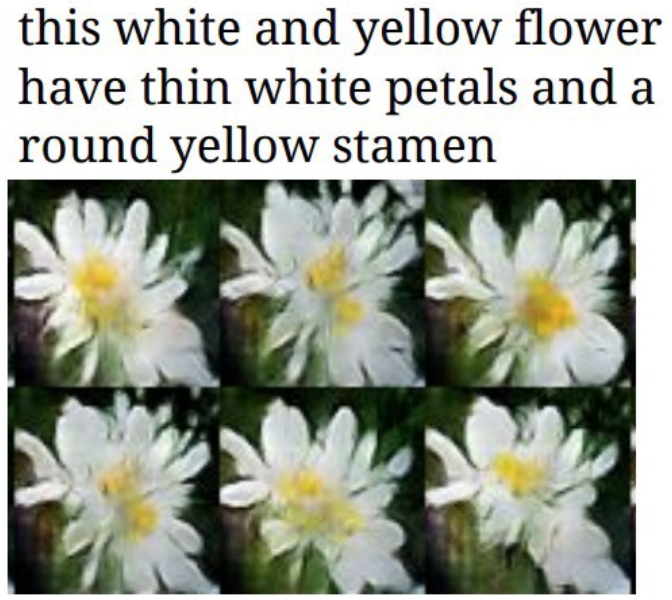
\includegraphics[width=0.3\textwidth]{fig/text_to_image.png}\hspace{1mm}
     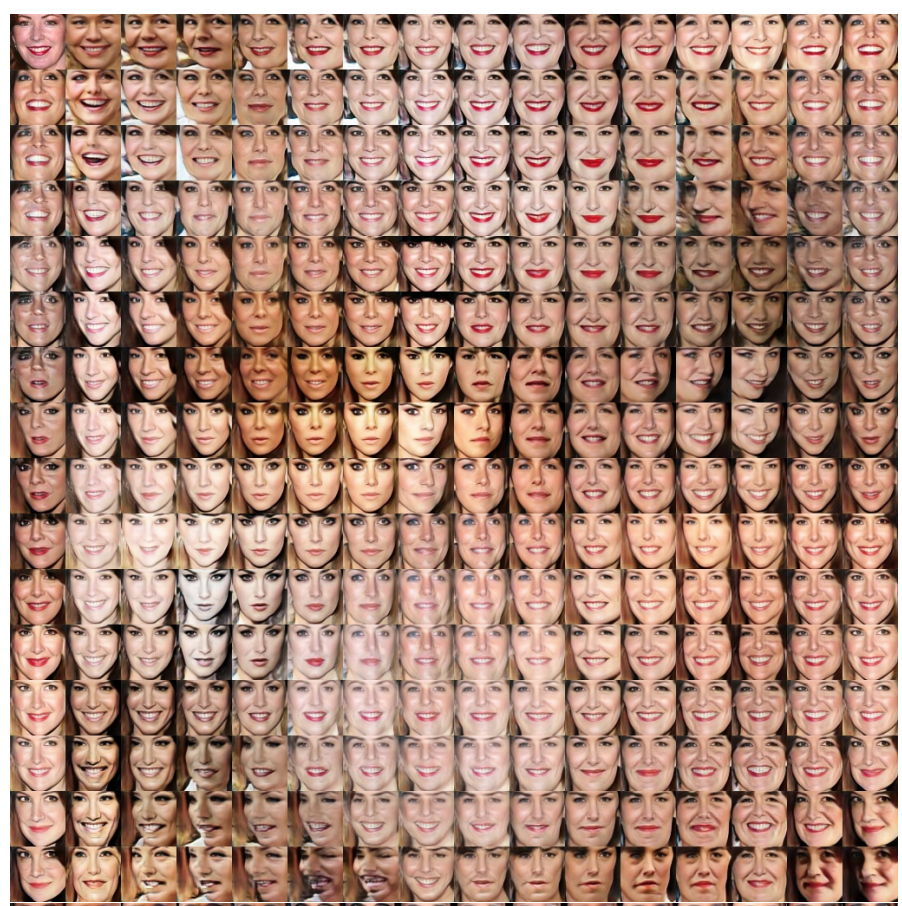
\includegraphics[width=0.3\textwidth]{fig/data_augm.png}\hspace{1mm}
      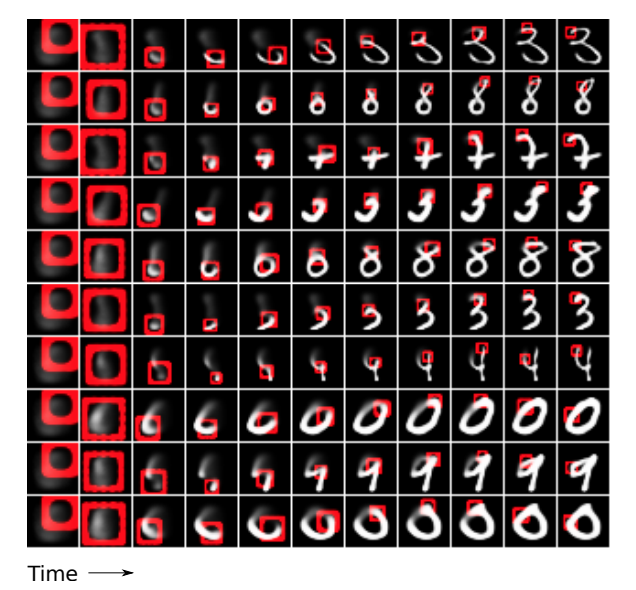
\includegraphics[width=0.3\textwidth]{fig/draw.png}
  \end{center}
  \caption{\cite{DBLP:journals/corr/ReedAYLSL16,2017arXiv171104340A,2015arXiv150204623G}}
\end{figure}


\end{frame}
%----------------------------------------------------------------------------------------

\begin{frame}
\frametitle{Probability measures and histograms}

Let $\Omega$ be a mesurable space.
\begin{itemize}
\item A probability measure is a measure $\mu$ on $\Omega$ such that $\int_{\Omega} d\mu=1$.
\item We note $\mathcal{P}(\Omega)$ the space of all probability measures on $\Omega$.
\end{itemize}

In the discrete case where  $\Omega=\{x_{1},..,x_{n}\}$ a probability mesure can be described through \emph{histograms} such that :

$$\mu=\sum_{i=1}^{n} \mu_{i} \delta_{x_{i}} $$

 where $\delta_{x_{i}}(x)=1$ if $x=x_{i}$ else $0$ and $\sum_{i=1}^{n} \mu_{i}=1$. $\mu_{i}$ is the probability of the event $x_{i}$. 


\end{frame}

%----------------------------------------------------------------------------------------

\begin{frame}
\frametitle{Probability measures and histograms}

\begin{itemize}
\item Bernouilli law : toss a coin $\Omega=\{\text{pile},\text{face}\}$ and $\mu_{i=1,2} \in \{0.5,0.5\}$
\item Color histograms in image : pixels as empirical distribution
\begin{figure}
  \begin{center}
    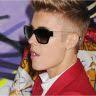
\includegraphics[width=0.22\textwidth]{fig/biber.png}\hspace{1mm}
     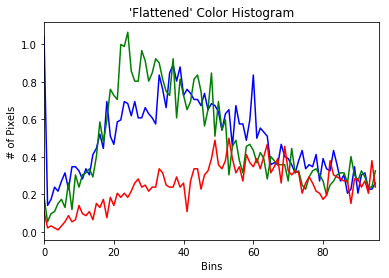
\includegraphics[width=0.42\textwidth]{fig/hist_biber.png}
  \end{center}
 \caption{Histogramme de Bieber}
\end{figure}
\item An image is a realization of a higher probability distribution where each pixel follows a distribution in the RGB color
\item Distribution of all the images of Bieber faces 
\end{itemize}
\end{frame}

%----------------------------------------------------------------------------------------

\begin{frame}
\frametitle{Everything leads to distributions: Empirical vs Histogram}

Many problems in which the output of the learning machine is both non-negative and multi-dimensional might be cast as predicting a measure

\normalsize\vspace{3mm}
Discrete measure: $\quad\displaystyle \mu=\sum_{i=1}^n \mu_i\delta_{\x_i},\quad
\x_i\in\Omega,\quad \sum_{i=1}^n \mu_i=1$
\begin{columns}[t]
\begin{column}{.45\linewidth}
\begin{block}{Lagrangian (point clouds)}\vspace{-3mm}
\begin{center}
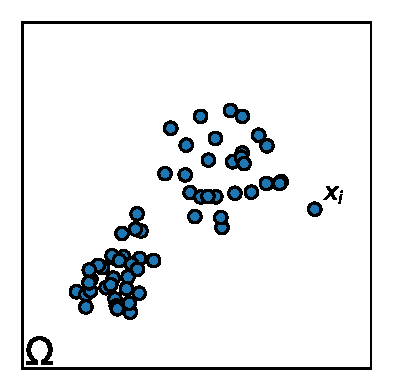
\includegraphics[width=.7\linewidth]{fig/distrib_empirical.pdf}
\end{center}\vspace{-5mm}
\begin{itemize}
\item Constant weight: $\mu_i=\frac{1}{n}$
\item Quotient space: $\Omega^n$, $\Sigma_n$ 
\end{itemize}
\end{block}
\end{column}
\begin{column}{.45\linewidth}
\begin{block}{Eulerian (histograms)}\vspace{-3mm}
\begin{center}
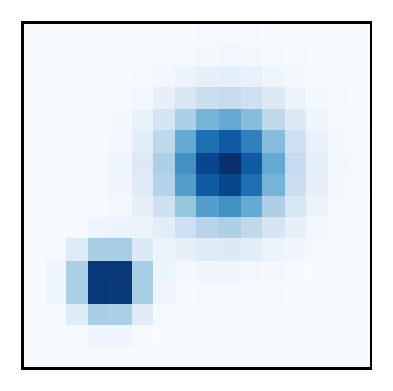
\includegraphics[width=.7\linewidth]{fig/distrib_hist.pdf}
\end{center}\vspace{-5mm}
\begin{itemize}
\item Fixed positions $\x_i$ e.g. grid
\item Convex polytope $\Sigma_n$ (simplex):
$\left\{(\mu_i)_i\geq 0; \sum_i \mu_i=1\right\}$
\end{itemize}
\end{block}
\end{column}
\end{columns}
\end{frame}

%----------------------------------------------------------------------------------------


\begin{frame}
\frametitle{Prerequisite : divergences}

In order two learn from distributions one needs to define a way to compare distributions. 

-> One possibility to achieve this is the notion of \emph{divergence} of distributions.

\pause 

$D: \mathcal{P}(\Omega) \times  \mathcal{P}(\Omega) \rightarrow \mathbb{R}$ is a divergence if it satisfies :

\begin{itemize}
\item for any distributions $P$ and $Q$, $D(P||Q) \geq 0$
\item $D(P||Q) = 0 \iff P=Q $ a.e
\end{itemize}

\pause 
Divergences are ways to define a similarity between distributions. They are not distances (may not be symmetric and no triangule inequality)

\end{frame}
%----------------------------------------------------------------------------------------

\begin{frame}
\frametitle{Kullback Leiber divergence}

If we have two distributions $P(x)$, $Q(x)$ over the same random variable $x$ we can define :

\begin{equation}
\label{kldiv}
\text{KL}(P||Q)=\underset{x \sim P}{\mathbb{E}}\big[\log(\frac{P(x)}{Q(x)})\big]=\int_{\Omega} \log(\frac{P(x)}{Q(x)}) P(x) dx
\end{equation}

KL it is the extra amount of information needed :

\begin{itemize}
\item To send a message containing symbols drawn from $P$,
\item When we use a code that was designed to minimize the length of messages drawn from $Q$.
\end{itemize}
  

\end{frame}
%----------------------------------------------------------------------------------------

\begin{frame}
\frametitle{Kullback Leiber divergence is asymetric}

\begin{figure}
  \begin{center}
    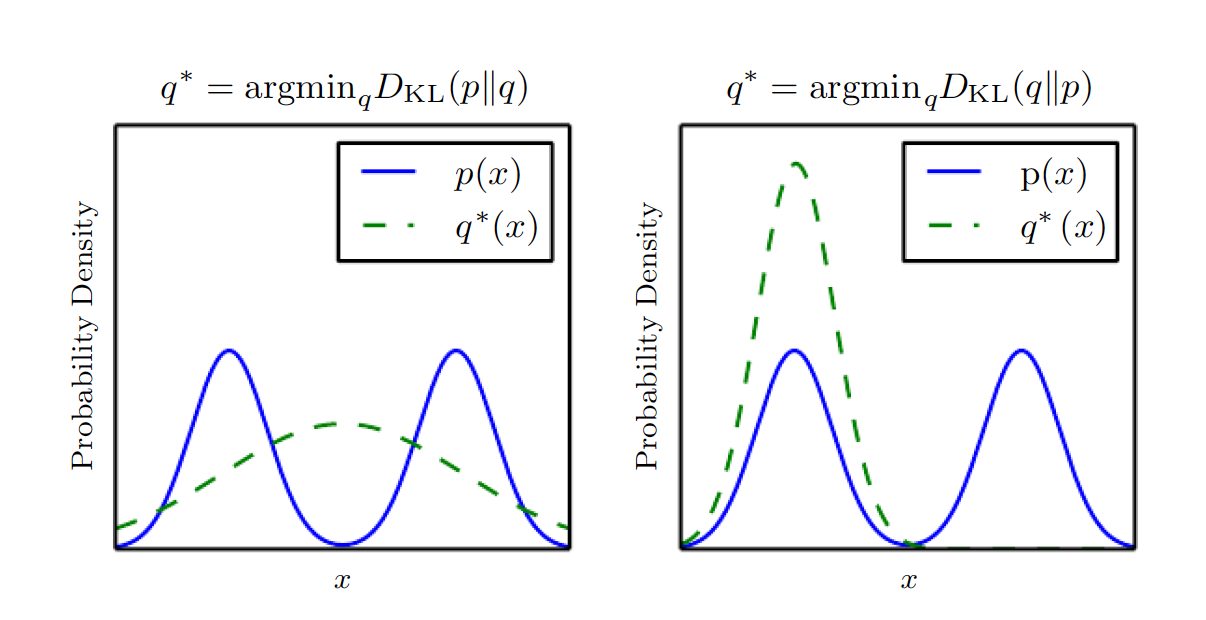
\includegraphics[width=0.7\textwidth]{fig/asymkl.png}
  \end{center}
  \caption{{\small Suppose we wish to approximate $p(x)$ with another distribution $q(x)$. (Left)The effect of minimizing $\text{KL}(p||q)$ : $q$ has high probability where $p$ has high probability. (Right)The effect of minimizing $\text{KL}(q||p)$ : $q$ has low probability where $p$ has low probability \cite{DBLP:journals/nature/LeCunBH15}}}
\end{figure}

We can derive the symetric Jensen-shannon divergence from the KL-divergence 
\begin{equation}
\label{kldiv}
\text{JSD}(P||Q)=\frac{1}{2} \text{KL}(P||P_{A}) + \frac{1}{2} \text{KL}(Q||P_{A})
\end{equation}
where $P_{A}=\frac{P+Q}{2}$
 
\end{frame}
%----------------------------------------------------------------------------------------

\begin{frame}
\frametitle{A lot of similarity measures...  \cite{Rubner2000}}

For discrete histograms with same number of bins $P=(p_{i})_{i}$,$Q=(q_{i})_{i}$ :

\begin{itemize}
\item Minkowski distance or $\ell_{p}$ distances : $d_{L_{r}}(P,Q)= \big(\sum_{i} |p_{i}-q_{i}|^{r}\big)^{\frac{1}{r}}$
\item Histogram intersection : $d_{h}(P,Q)= 1-\frac{\sum_{i} \text{min}(p_{i},q_{i})}{\sum_{i}q_{i}}$
\item$\chi^{2}$ statistic : $d_{\chi^{2}}(P,Q)= \sum_{i} \frac{(p_{i}-q_{i})^{2}}{h_{i}}$, where $m_{i}=\frac{p_{i}+q_{i}}{2}$
\item Quadratic form distance : $d_{A}(P,Q)=\sqrt{(P-Q)^{T} A (P-Q)}$ with $A=(a_{ij})$ the "cross-bin" information.
\item Kolmogorov-Smirnov distance, match distance ...
\end{itemize}

\pause 

How to choose ? Each one has its advantages and its drawbacks (some clues coming...)

\pause 
Now that we now how to compare distributions how do we learn them ?

\end{frame}

%----------------------------------------------------------------------------------------

\begin{frame}
\frametitle{Classical Log likehood approach}

Usually to learn a distribution $\mathbb{P}_{r}$ we use a parametric family of densities $(\mathbb{P}_{\theta})_{\theta \in \Theta}$ and try to maximize the following log-likehood  :

\begin{equation}
\label{loglike}
 \underset{\theta \in \Theta}{\text{max}} \ \underset{x \sim \mathbb{P}_{r} }{\mathbb{E}}[\log(P_{\theta}(x))] \approx \underset{\theta \in \Theta}{\text{max}} \ \frac{1}{m} \sum_{i=1}^{m} \log P_{\theta}(x_{i})
 \end{equation}

Example : gaussian mixture, logistic regression where we want to learn the distribution $P(Y=1|X=x)$ using the parametric family $(\sigma(\theta^{T} x))_{\theta \in R^{d}}$...

\begin{center}
\movie[autostart,repeat]{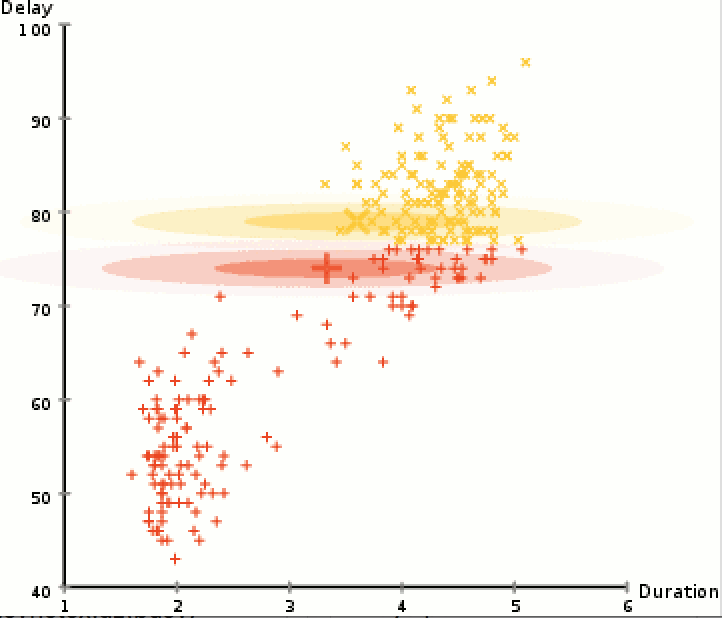
\includegraphics[width=0.5\textwidth]{fig/fitting0.png}}{fig/fitting.mov}
\end{center}

\end{frame}
%----------------------------------------------------------------------------------------

\begin{frame}
\frametitle{Classical Log likehood approach}

\begin{block}{Asymptotic behavior}
If $\mathbb{P}_{r}$ has a density, and $\mathbb{P}_{\theta^{*}}$ is the density maximizing \eqref{loglike} then asymptotically $\mathbb{P}_{\theta^{*}}$ is such that : 
$$\text{KL}(\mathbb{P}_{r}||\mathbb{P}_{\theta^{*}})= \underset{\theta \in \Theta}{\text{min}} \ \text{KL}(\mathbb{P}_{r}||\mathbb{P}_{\theta})$$

Solving \eqref{loglike} is equivalent to find the "closest" distribution amoung the given parametric family which fits the target distribution (\textit{w.r.t} the KL-divergence)
\end{block}


\end{frame}
%----------------------------------------------------------------------------------------

\section{Original GAN \cite{googfellow2014}}
%----------------------------------------------------------------------------------------

\begin{frame}
\frametitle{Generative model}

\begin{block}{Generative problem}
We want to construct a distribution $\mathbb{P}_{g}$, called a generative distribution, which mimicks the real distribution $\mathbb{P}_{r}$.
\end{block}

\begin{figure}
  \begin{center}
    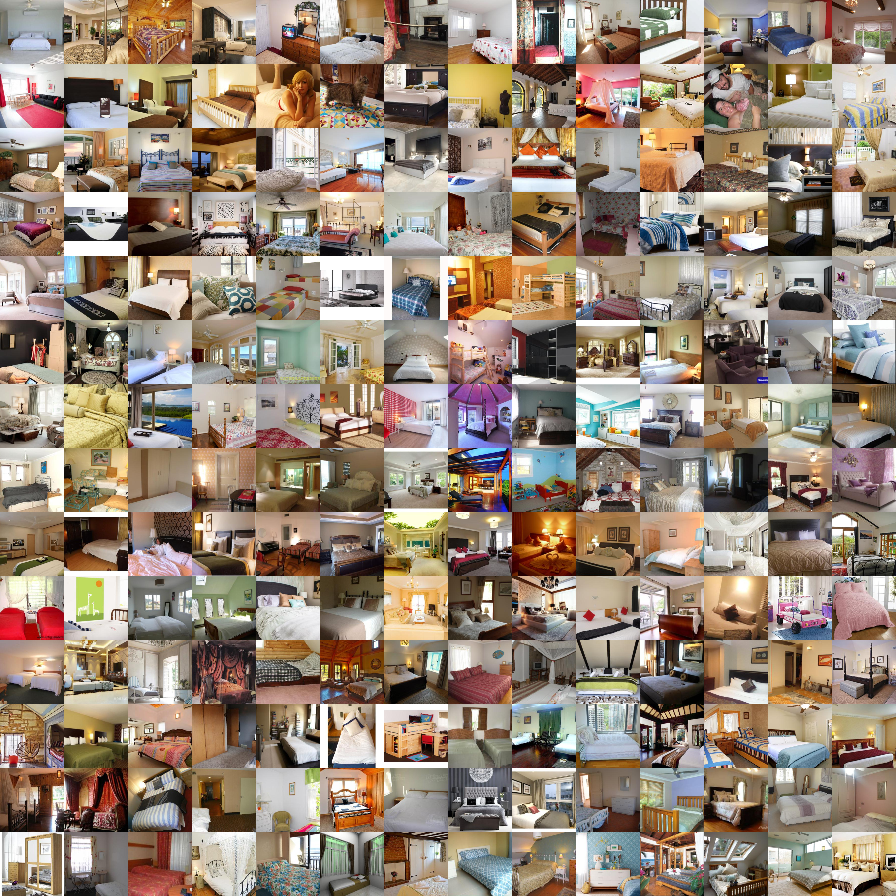
\includegraphics[width=0.5\textwidth]{fig/lsun_bedrooms_real.png}\hspace{1mm}
     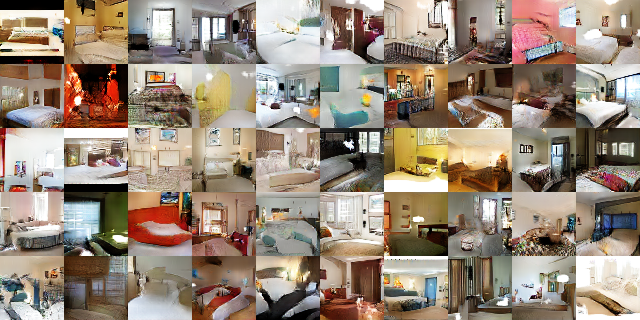
\includegraphics[width=0.45\textwidth]{fig/lsun_bedrooms_five_epoch_samples.png}\hspace{1mm}
  \end{center}
  \caption{\cite{2015arXiv151106434R}}
\end{figure}

\end{frame}
%----------------------------------------------------------------------------------------

\begin{frame}
\frametitle{The adverserial Setting}
Neural networks that perform at human level accuracy have a nearly 100\% error rate on examples that are intentionally constructed to fool the network. 

For \textit{e.g} by searching an input $x'$ near a data point $x$ such that the model output is very different at $x'$ : it is \emph{adversarial examples} \cite{2014arXiv1412.6572G} 

\begin{figure}
  \begin{center}
    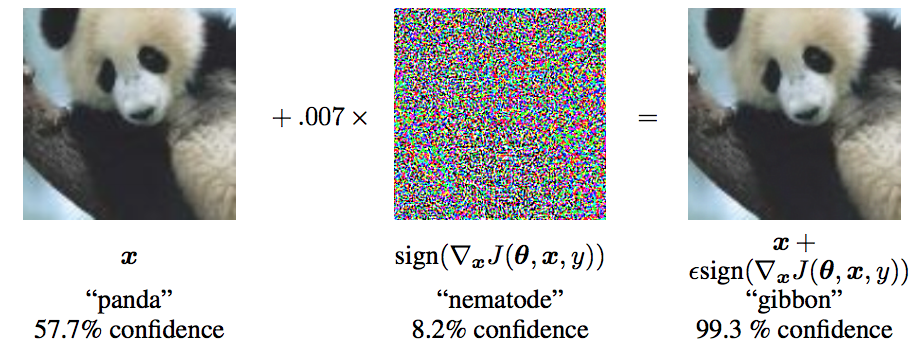
\includegraphics[width=0.7\textwidth]{fig/gibon.png}
  \end{center}
\end{figure}


\end{frame}
%----------------------------------------------------------------------------------------

\begin{frame}
\frametitle{Problem setting}

In this approach, a generative model (the \emph{generator}) is trained to learn $\mathbb{P}_{g}$ by fooling a feedforward classifier (the \emph{discriminator}):
\begin{itemize}
\item The discriminator attempts to recognize all samples from the generative model as being fake, and all samples from the training set as being real.
\pause
\item Based on a game theoretic scenario in which the generator network must compete against the discriminator (\url{https://en.wikipedia.org/wiki/A_Beautiful_Mind_(film)}) :

\pause 

A function $L(G ,D)$ determines the payoff of the discriminator. The generator receives $-L(G ,D)$ as its own payoff. Each player attempts to maximize its own payoff :

$$\underset{D}{\text{max}} \ \underset{G}{\text{min}} \ L(G ,D)$$

\end{itemize}

What is $L$ ?

\end{frame}

%----------------------------------------------------------------------------------------

\begin{frame}
\frametitle{Problem setting}

In the most classical GAN setting we have to solve the following problem :

\begin{equation}
\label{ganoriginalproblem}
\underset{D}{\text{max}} \ \underset{G \ \text{produces} \  \mathbb{P}_{g}}{\text{min}} \  \ \underset{x \sim \mathbb{P}_{r}}{\mathbb{E}}[\log(D(x))]+ \underset{x' \sim \mathbb{P}_{g}}{\mathbb{E}}[\log(1-D(x'))]
\end{equation}

\begin{itemize}
\pause 
\item $\underset{D}{\text{max}} \underset{x \sim \mathbb{P}_{r}}{\mathbb{E}}[\log(D(x))]+ \underset{x' \sim \mathbb{P}_{g}}{\mathbb{E}}[\log(1-D(x'))]$ : force $D$ to differientiate all sample from $\mathbb{P}_{r}$ and from $ \mathbb{P}_{g}$
\pause
\item $\underset{G \ \text{produces} \  \mathbb{P}_{g}}{\text{min}}  \underset{x' \sim \mathbb{P}_{g}}{\mathbb{E}}[\log(1-D(x'))]$ :  the generator learns to fool $D$
\end{itemize}

\pause

This raise two questions : how do we model "$G \ \text{produces} \  \mathbb{P}_{g}$" and how do we model $D$ ??


\end{frame}
%----------------------------------------------------------------------------------------

\begin{frame}
\frametitle{How to model the generator G : latent variable }

\begin{itemize}
\item The more complicated the dependencies between the dimensions, the more difficult the models are to train. 
\pause
\item For \textit{e.g} if we care about modeling the digits $0-9$. If the left half of the character contains the left half of a $5$, then the right half cannot contain the left half of a $0$.
\pause
\item This a priori helps if the model first decides which character to generate before it assigns a value to any specific pixel
\end{itemize}

\pause
This kind of decision is called a \emph{latent variable} : before our model draws anything, it first randomly samples a digit value.

\begin{figure}
  \begin{center}
    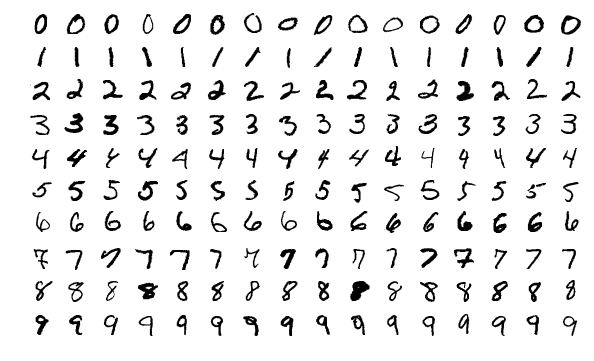
\includegraphics[width=0.6\textwidth]{fig/mnist.png}
  \end{center}
\end{figure}

\end{frame}

%----------------------------------------------------------------------------------------

\begin{frame}
\frametitle{How to model the generator G : latent variable }

Let $\mathcal{X}$ be the space of the data. 
\begin{itemize}
\item We have a latent space $\mathcal{Z}$ which we can sample to using some probability density $p(z)$. (typically gaussian noise)
\item  We then use parametric functions $g_{\theta} : \mathcal{Z} \rightarrow \mathcal{X}$.  
\item $g_{\theta}$ is now a random variable in the space of our data $\mathcal{X}$
\end{itemize}

The goal is to to optimize $\theta$ such that we can sample $z$ from $p(z)$ and, with high probability, $g_{\theta}(z)$ will be like the X’s in our dataset.

\begin{figure}
  \begin{center}
    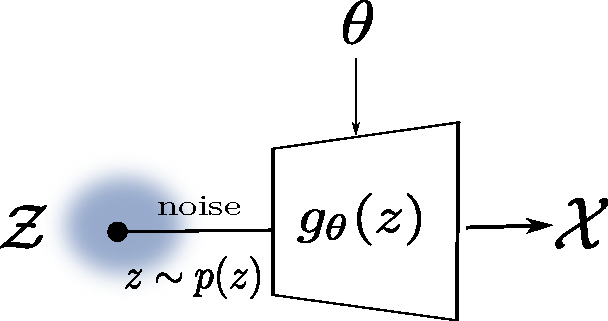
\includegraphics[width=0.6\textwidth]{fig/latent.pdf}
  \end{center}
\end{figure}

\pause 
What parametric family $g_{\theta}$ do we choose ? -> neural network

\end{frame}

%----------------------------------------------------------------------------------------

\begin{frame}
\frametitle{Why using neural network ?}

\begin{block}{Representer theorem}
Let $g$ be a bounded, continuous and non decreasing (activation) function. Let $K_{d}$ be some compact set in $R_{d}$ and $C(K_{d})$ the set of continuous functions on $K_{d}$ . Let $f \in C(K_{d})$. 

Then for all $\epsilon > 0$, there exists $N \in \mathbb{N}$, real numbers $v_{i}, b_{i}$ and $R_{d}$vectors $w_{i}$ such that the function
$$F(x) = \sum_{i=1}^{N} v_{i} g( \langle w_{i},x\rangle  +b)$$
satisfies
$\forall x \in K_{d}, \ | F(x) - f(x) | \leq \epsilon$

\end{block}
\end{frame}
%----------------------------------------------------------------------------------------

\begin{frame}

\frametitle{Putting everything together}

We use a neural network $G=g_{\theta}$ and a noise $p(z)$ such that $x'=g_{\theta}(z), z \sim p(z)$ :

\begin{equation}
\label{ganeeq}
\underset{D}{\text{max}} \ \underset{g_{\theta}}{\text{min}} \  L(D,g_{\theta}) = \underset{x \sim \mathbb{P}_{r}}{\mathbb{E}}[\log(D(x))]+ \underset{z \sim p(z)}{\mathbb{E}}[\log(1-D(g_{\theta}(z)))]
\end{equation}

The discriminator is also au neural network.

\begin{figure}
  \begin{center}
    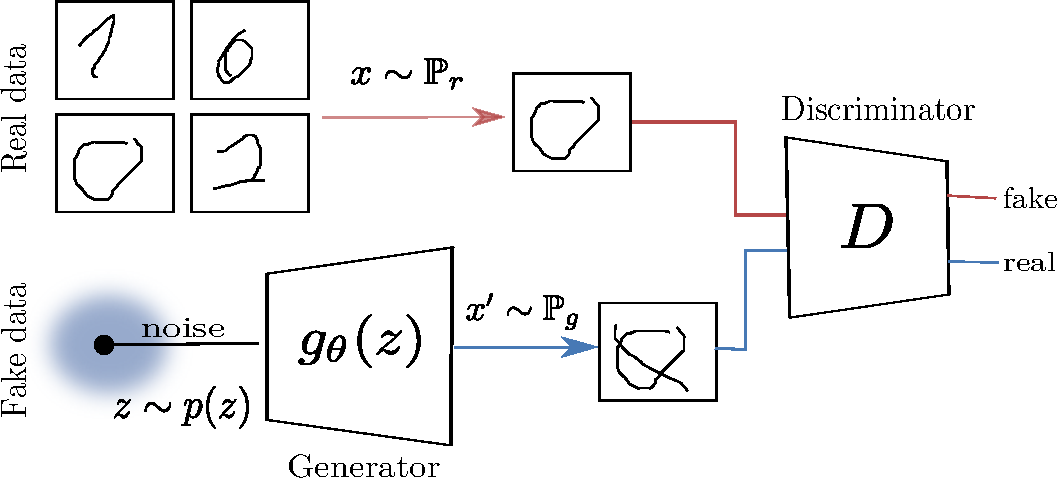
\includegraphics[width=0.9\textwidth]{fig/gan.pdf}
  \end{center}
\end{figure}

\end{frame}
%----------------------------------------------------------------------------------------

\begin{frame}
\frametitle{Theoretical results}

To solve this problem we use alternate updates of $D$ and $G$ by iterating the two following steps :
\begin{itemize}
\item First train the discriminator $D$ by maximizing \eqref{ganeeq} \textit{w.r.t} $D$
\item Train the generator $G$ by minimizing  \eqref{ganeeq} \textit{w.r.t} $G$
\end{itemize}

One can show that the first step (with generator fixed)  leads to an optimal discriminator : $$D^{*}(x)= \frac{\mathbb{P}_{r}(x)}{\mathbb{P}_{r}(x)+\mathbb{P}_{g}(x)}$$ 
The second step is equivalent at finding the generator which minimizes : 
\begin{equation}
\label{jsdeq}
2 \text{JSD}(\mathbb{P}_{r},\mathbb{P}_{g})-2\log 2 
\end{equation}
 so that we have :
 \begin{block}{Solution to \eqref{ganeeq}}
The global minimum of \eqref{ganeeq} is achieved if and only if $\mathbb{P}_{r}=\mathbb{P}_{g}$ and at that point  $L(D^{*},G^{*})=-2\log 2$
\end{block}

\end{frame}


%----------------------------------------------------------------------------------------


\begin{frame}
\frametitle{Implementation of GAN}

        \begin{algorithm}[H]   
            \begin{algorithmic}[1]
                \STATE {Discriminator with parameters $\theta_{d}$ and generator with parameters $\theta_{g}$}

                \FOR {number of training iterations}
                \FOR{$k$ steps}
                \STATE {sample minibatches $\{z_{1},...,z_{m}\}$  from noise prior $p(z)$}
                \STATE {sample minibatches $\{x_{1},...,x_{m}\}$  from data $\mathbb{P}_{r}$}
                \STATE {Update the discriminator  by ascending its stochastic gradient $$\nabla_{\theta_{d}} \frac{1}{m} \sum_{i=1}^{m} \log[D(x_{i})]+\log[1-D(\g_{\theta_{g}}(z_{i}))]  $$}
                \ENDFOR

                \STATE {sample minibatches $\{z_{1},...,z_{m}\}$  from noise prior $p(z)$}
                \STATE {Update the generator  by ascending its stochastic gradient $$\nabla_{\theta_{g}} \frac{1}{m} \sum_{i=1}^{m} \log[1-D(\g_{\theta_{g}}(z_{i}))]  $$}
                \ENDFOR
            \end{algorithmic}
                      \caption{\label{gan} pseudo code of GAN}
        \end{algorithm}


\end{frame}
%----------------------------------------------------------------------------------------

\begin{frame}
\frametitle{How to build the discriminator and generator ? }
One rule : don't be a hero. There exist a lot of GAN architectures : GAN, AC-GAN, BiGAN, BGAN, CC-GAN, CGAN (conditionnal)

 We will focus on the classicals GAN (\cite{googfellow2014}) and DCGAN (\cite{2015arXiv151106434R}) :
 
 \begin{itemize}
 \item Original GAN doesn't use convolution : only dense layer with ReLu/sigmoid/maxout activation and batch normalization
 \item DCGAN :
 \begin{figure}
  \begin{center}
    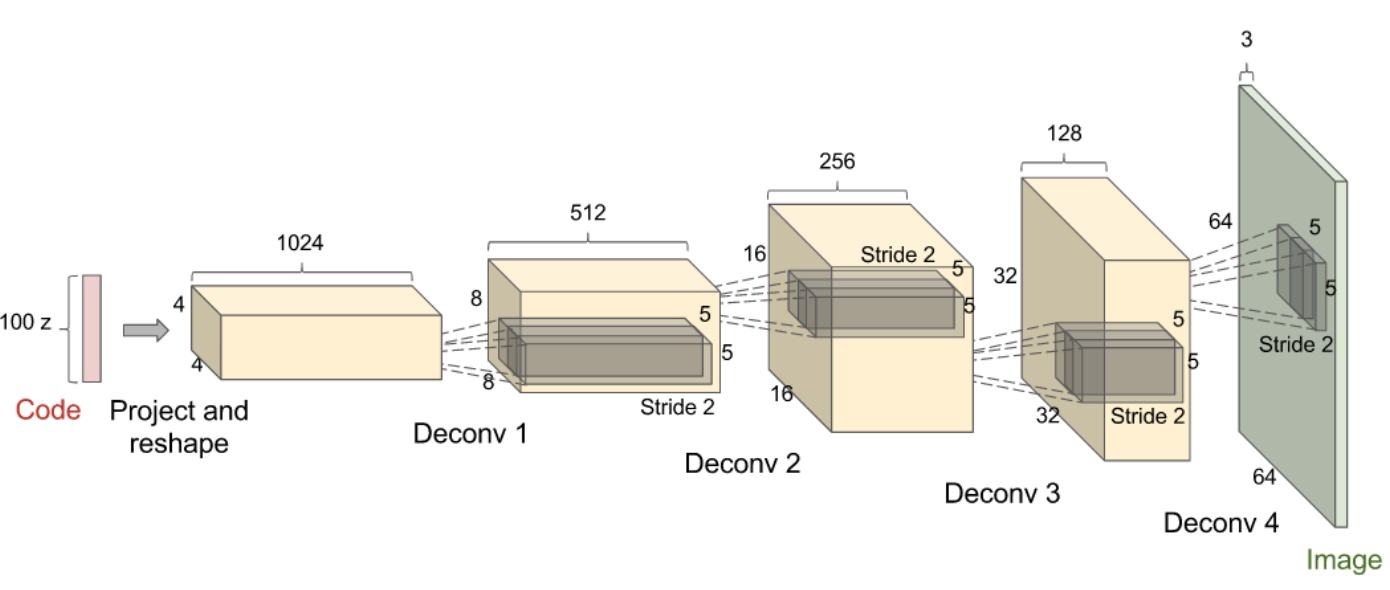
\includegraphics[width=0.9\textwidth]{fig/dcgan_generator.png}
  \end{center}
\end{figure}
 \end{itemize}
 

\end{frame}
%----------------------------------------------------------------------------------------

\begin{frame}
\frametitle{DCGAN}

\begin{itemize}
\item Replace any pooling layers with strided convolutions : the generator needs to increase the spatial dimension of the representation.
\item Use Batch Normalization in both the generator (except at the output layer) and the discriminator (except at the input layer)
\item Remove fully connected hidden layers for deeper architectures
\item Use ReLU activation in generator for all layers except for the output
\item Use LeakyReLU activation in the discriminator for all layers
\end{itemize}

\end{frame}
%----------------------------------------------------------------------------------------

\begin{frame}
\frametitle{Downside of traditional GAN's}

GAN training is theoretically guaranteed to converge if we can modify the density functions directly, but:

\begin{itemize}
\item Instead, we modify G and D  : have they enough capacity to represent the distributions ?
\item  G and D are highly non-convex parametric functions
\item “Oscillation”: can train for a very long time, generating very many different categories of samples, without clearly generating better samples
\end{itemize}

\end{frame}

%----------------------------------------------------------------------------------------


\begin{frame}
\frametitle{Mode collapse or mode dropping : most severe form of non convergence}
GAN's fail to learn the entire distribution but just modes of the distribution.

\begin{itemize}
\item When training D : convergence to the correct "best" distribution
\item When training G in the inner loop : place all mass on most likely points
\end{itemize}
 \begin{figure}
  \begin{center}
    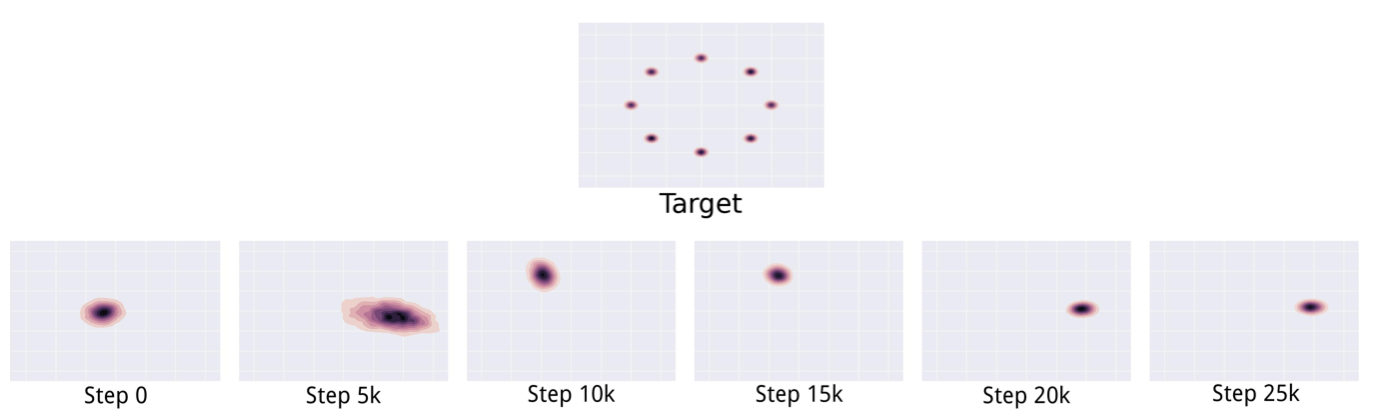
\includegraphics[width=0.9\textwidth]{fig/mode_collapse}
  \end{center}
\end{figure}
\end{frame}

%----------------------------------------------------------------------------------------

\begin{frame}
\frametitle{What is the core of mode dropping ?}

Getting back to the $\text{KL}$ divergence :

$$\text{KL}(\mathbb{P}_{r}||\mathbb{P}_{g})= \int_{\mathcal{X}} P_{r}(x) \log \frac{ P_{r}(x)}{ P_{g}(x)} dx$$

\begin{itemize}
\item If $P_{r}(x) > P_{g}(x)$, then $x$ is a point with higher probability of coming from the data than being a generated sample.
\item Mode dropping is when there are large regions with high values of $P_{r}$, but small or zero values in $P_{g}$.
\item The integrand inside the KL grows quickly to infinity :  the $\text{KL}$ cost assigns an extremely high cost to a generator’s distribution not covering parts of the data.
\end{itemize}

In practice the $\text{KL}$ divergence occurs in training GAN's so that this situation happens.


\end{frame}


%----------------------------------------------------------------------------------------


\begin{frame}
\frametitle{Mode collapse causes low output diversity}
 \begin{figure}
  \begin{center}
    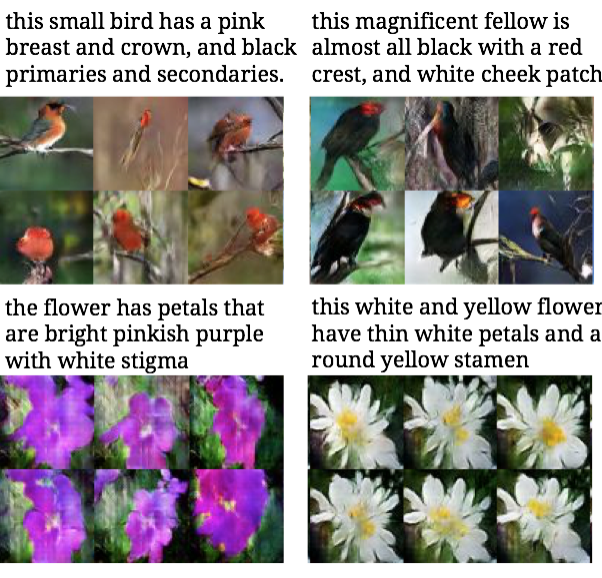
\includegraphics[width=0.7\textwidth]{fig/diversity}
  \end{center}
\end{figure}
\end{frame}



%----------------------------------------------------------------------------------------
\begin{frame}
\frametitle{Why ? Some enlightening responses \cite{arjovsky_towards_2017}}

First reason : the distributions $\mathbb{P}_{r}$ and $\mathbb{P}_{g}$ lie on small dimensional subsets that don't intersect so that $\text{KL}$ divergences are undefined.

\pause

In theory : the trained discriminator have cost at most $2 \log 2 - 2 \text{JSD}(\mathbb{P}_{r}||\mathbb{P}_{g})$.
\begin{itemize}
\item  In practice, if we just train D till convergence, its error will go to 0
\item The only way this can happen is if the distributions are not continuous, or they have disjoint supports.
\end{itemize}


\end{frame}



\begin{frame}
\frametitle{Why ? Some enlightening responses \cite{arjovsky_towards_2017}}



\begin{block}{Theorem}

Let $\mathbb{P}_{r}$ and $\mathbb{P}_{g}$ be two distributions whose support lies in two manifolds that don’t have full dimension and don’t perfectly align. Then :
\begin{itemize}
\item $\text{JSD}(\mathbb{P}_{r}||\mathbb{P}_{g})=\log 2$
\item $\text{KL}(\mathbb{P}_{r}||\mathbb{P}_{g})=\infty$
\item $\text{KL}(\mathbb{P}_{g}||\mathbb{P}_{r})=\infty$
\end{itemize}
\end{block}

\pause

Use this divergences to test similarities between the distributions is a terrible : these divergencies are always maxed out -> minimizing them by gradient descent isn’t really possible. 

Yet \eqref{jsdeq} shows that the generator step is minimizing a $\text{JSD}$

\end{frame}

\begin{frame}
\frametitle{Why ? Some enlightening responses \cite{arjovsky_towards_2017}}

Second reason : vanishing gradients

\begin{block}{Theorem}
Let $g_{\theta} : \mathcal{Z} \rightarrow \mathcal{X}$ be be a differentiable function that induces a distribution $\mathbb{P}_{g}$. Let $\mathbb{P}_{r}$ be the real data distribution. Suppose that the supports lies in two manifolds that don’t have full dimension and don’t perfectly align. Let $D$ be a differentiable discriminator. Then :

$$\underset{\|D-D^{*}\| \rightarrow 0}{\lim} \nabla_{\theta} \underset{z\sim p(z)}{\mathbb{E}}[\log(1-D(g_{\theta}(z))]=0  $$ 

\end{block}

\pause

\begin{itemize}
\item As our discriminator gets better, the gradient of the generator vanishes.
\item This makes it difficult to train using this cost function : decide the precise amount of training dedicated to the discriminator before the vanishing effect.
\end{itemize}


\end{frame}

\begin{frame}
\frametitle{The $-\log D$ alternative}
Instead of considering $ \underset{z \sim p(z)}{\mathbb{E}}[\log(1-D(g_{\theta}(z)))]$ we rather consider :

\begin{equation}
\label{ganeeqstab}
\underset{D}{\text{max}} \ \underset{g_{\theta}}{\text{min}} \  L(D,g_{\theta}) = \underset{x \sim \mathbb{P}_{r}}{\mathbb{E}}[\log(D(x))]+ \underset{z \sim p(z)}{\mathbb{E}}[-\log(D(g_{\theta}(z)))]
\end{equation}

\begin{itemize}
\item Doesn’t necessarily suffer from vanishing gradients : more stable cost function
\item Still suffers from mode dropping
\end{itemize}


\end{frame}



\begin{frame}
\frametitle{Evaluation of GAN's}


There is not a good way to quantify how good samples are : about 24 quantitative and 5 qualitative measures.

\pause

Most widely adopted : Inception Score. 
\begin{itemize}
\item It uses a pre-trained neural network (Inception Net) to capture the desirable properties of generated samples by running a classification on them 
\item We desire \emph{highly classifiable} and \emph{diversity} of the samples : expected to have low entropy for easily classifiable samples and high entropy on the classes.
\end{itemize}

\pause

$$\text{IS}=\exp(H(y)-\mathbb{E}_{x}[H(y|x)])$$

 where $y$ denote the classes and $x$ the samples.


\end{frame}
%----------------------------------------------------------------------------------------

\begin{frame}
\frametitle{Evaluation of GAN's \cite{DBLP:journals/corr/abs-1802-03446}}

\begin{figure}
  \begin{center}
    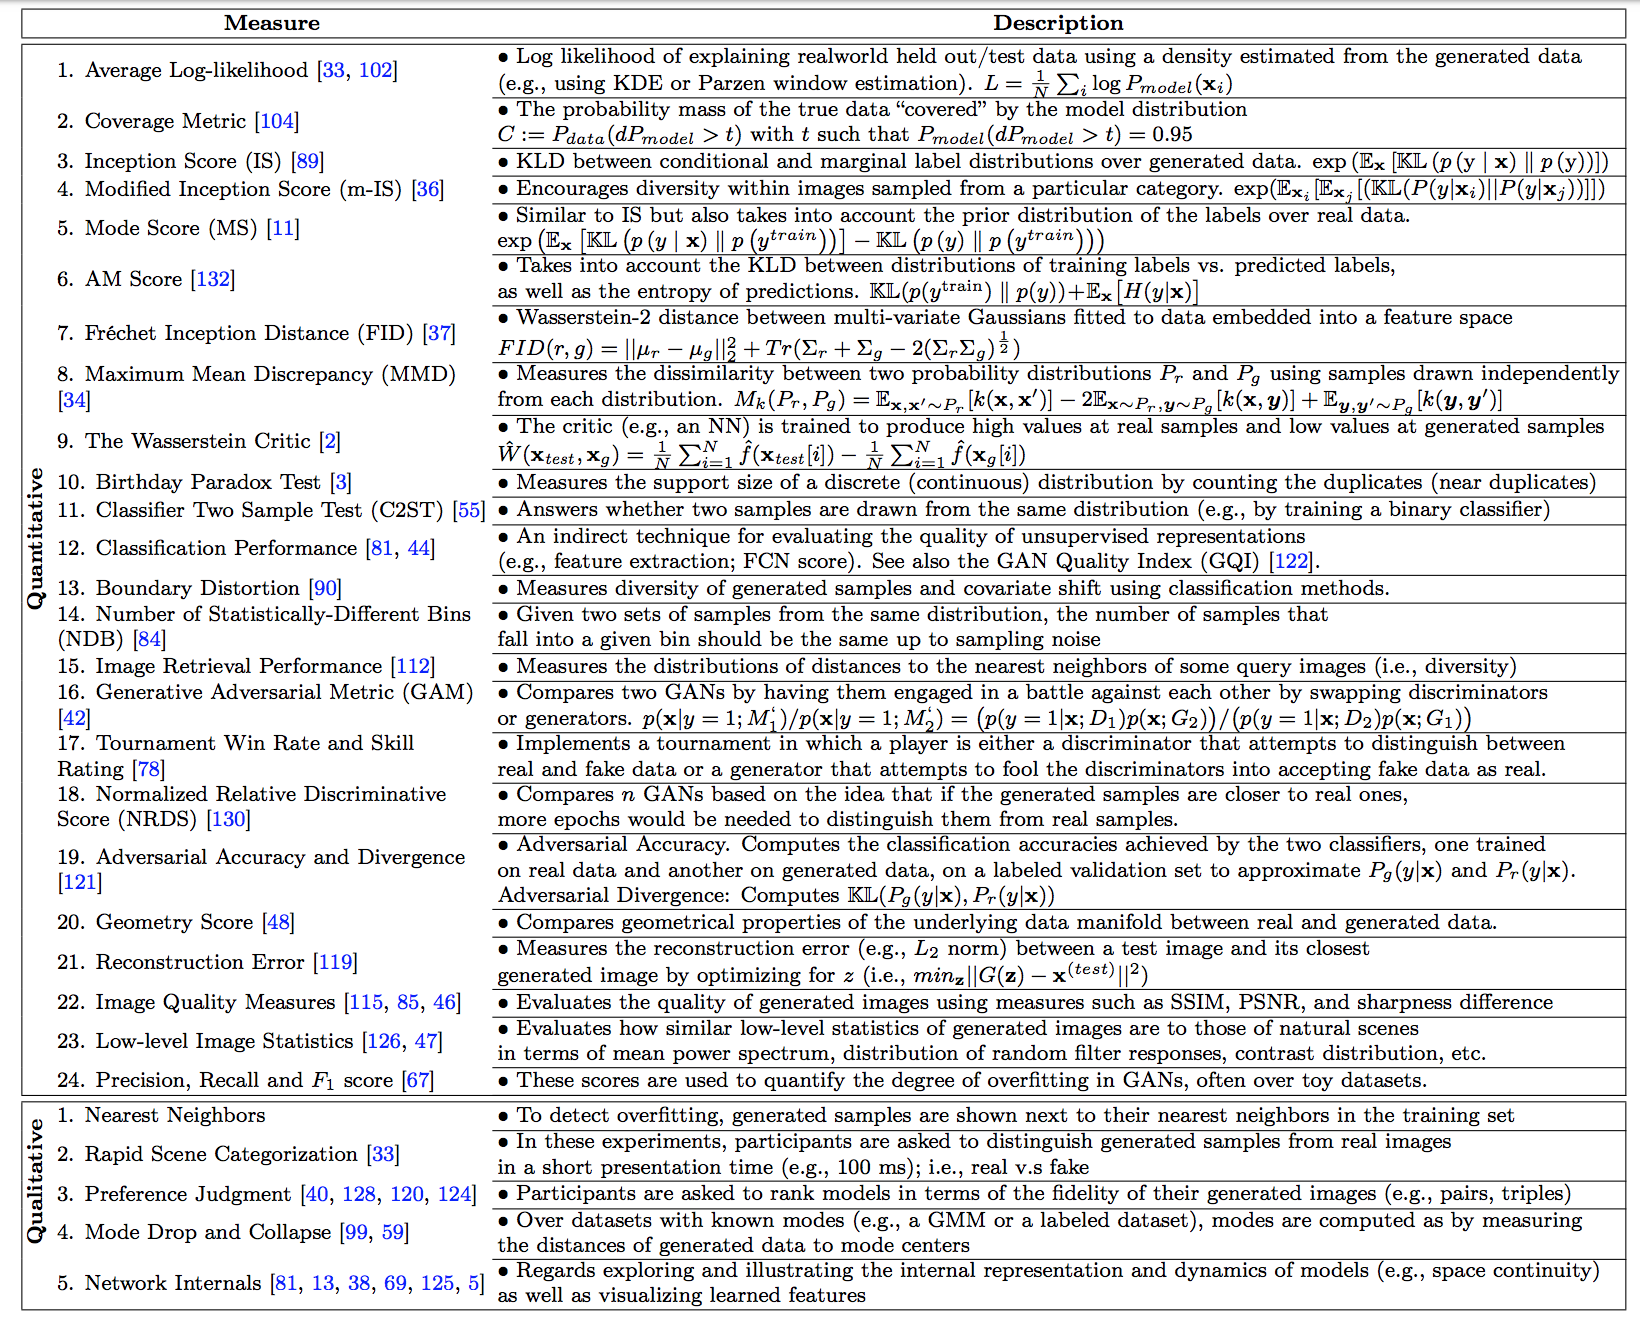
\includegraphics[width=0.95\textwidth]{fig/evaluation_gan.png}
  \end{center}
\end{figure}
\end{frame}
%----------------------------------------------------------------------------------------


%----------------------------------------------------------------------------------------

\section{Wasserstein GAN's}

\subsection{Optimal transport and Wasserstein distance}
%----------------------------------------------------------------------------------------

\begin{frame}
\frametitle{The origins of optimal transport}

\begin{center}
\only<1>{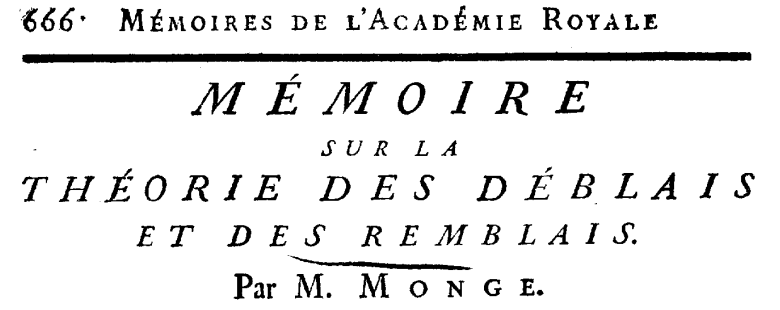
\includegraphics[width=0.7\linewidth]{fig/memoire_monge.png}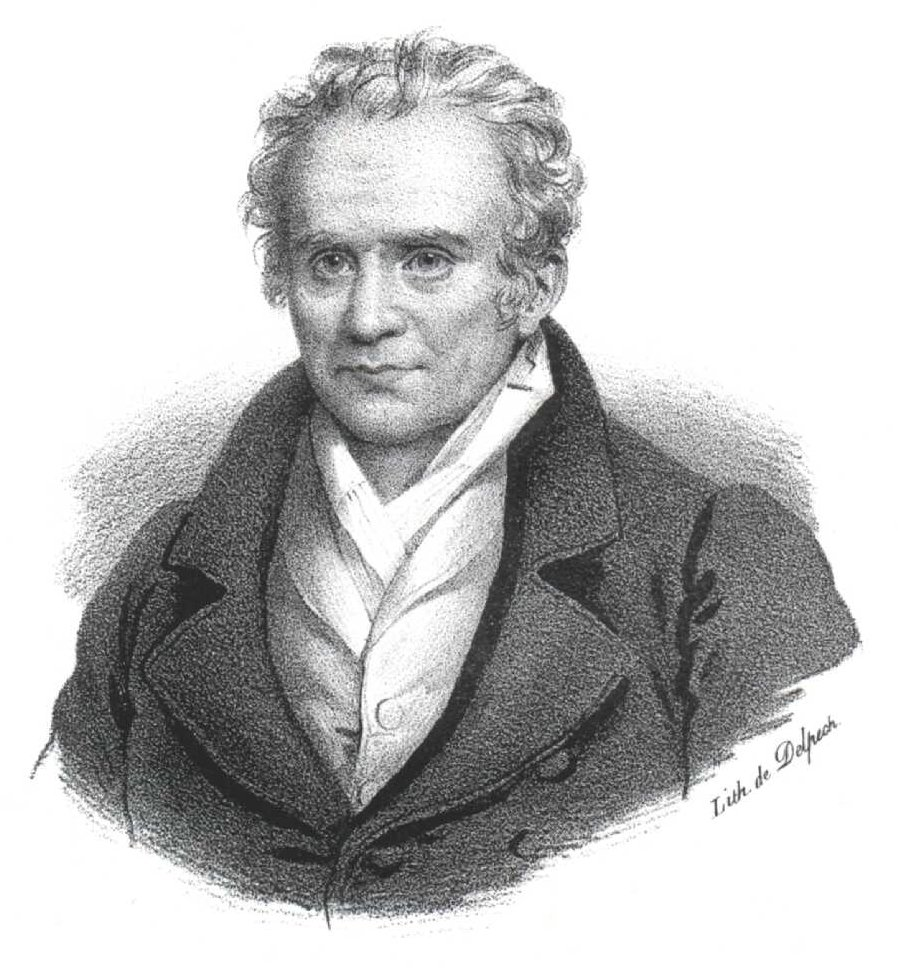
\includegraphics[width=0.25\linewidth]{fig/monge.jpg}}
\only<2>{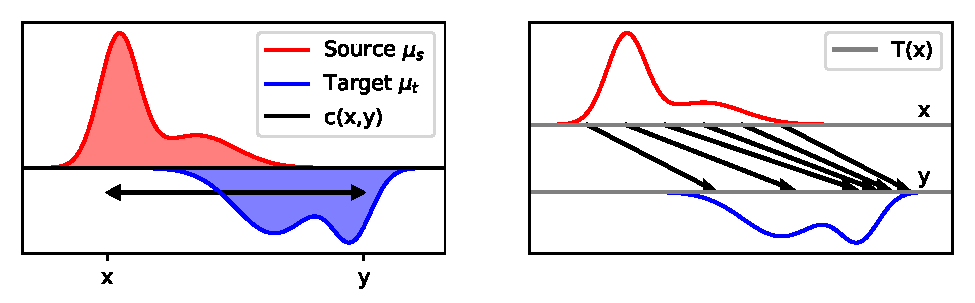
\includegraphics[width=0.9\linewidth]{fig/deblais_monge.pdf}}
\end{center}

\begin{block}{Problem}
\begin{itemize}
\item How to move dirt from one place (déblais) to another (remblais) while minimizing the effort ?
\item Find a mapping $T$ between the two distributions of mass (transport).
\item Optimize with respect to a displacement cost $c(x,y)$ (optimal).
\end{itemize}
\end{block}


\end{frame}

%----------------------------------------------------------------------------------------


\begin{frame}
  \frametitle{Optimal transport (Monge formulation)}

  \begin{itemize}
  \item Mathematical tools aiming at comparing distributions
    \begin{center}
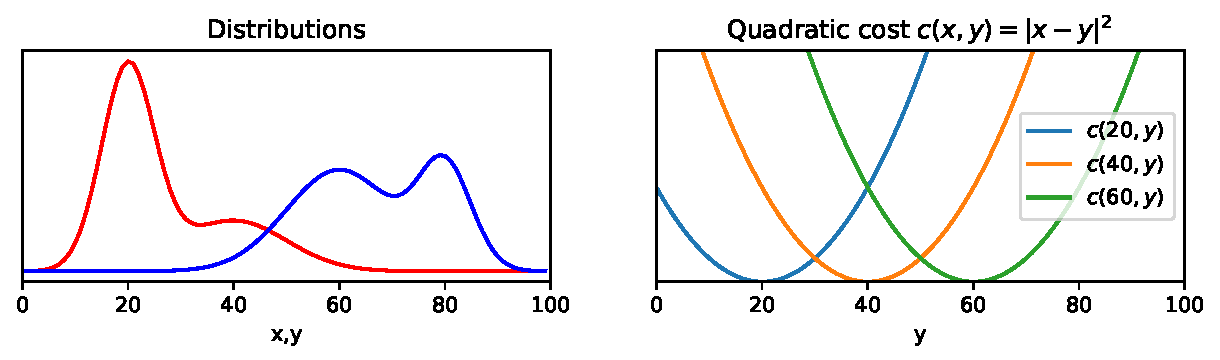
\includegraphics[width=0.9\linewidth]{./fig/dist_monge.pdf}  
\end{center}

  \item Probability measures $\red{\mu_s}$ and $\blue{\mu_{t}}$ on $\Omega_s$, $\Omega_t$    
    with a cost function
    $d: \Omega_{s} \times \Omega_{t} \rightarrow \mathbb{R}^{+}$.

  \item The Monge formulation aim at finding a mapping
    $T:\Omega_{s}\rightarrow \Omega_{t}$
    \begin{equation}
      \label{eq:1}
      \inf_{T\#\red{\mu_{s}}=\blue{\mu_{t}}}\quad\int_{\Omega_{s}} d(x,T(x))\red{\mu_{s}}(x)dx
    \end{equation}

  \end{itemize}
  

\end{frame}
%----------------------------------------------------------------------------------------


\begin{frame}
  \frametitle{What is $T\#\mu_s=\mu_t$ ?}
  \begin{center}
    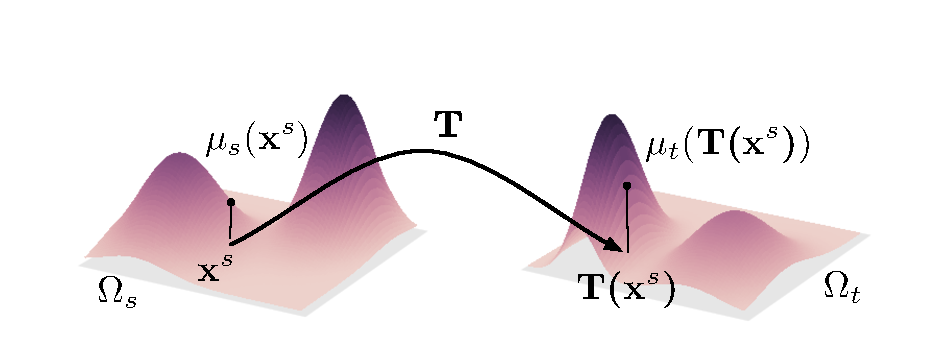
\includegraphics[width=0.7\linewidth]{fig/T}
  \end{center}

\begin{itemize}
\item $T\#$ is the so called push forward operator
\item it transfers measures from one space $\Omega_s$ to another space $\Omega_t$
\item it is equivalent to:
\begin{align*}
\mu_t(A) & =  \mu_s(T^{-1}(A))\\
\end{align*}
\item consists simply in moving the positions of all the points in the support of the measure :
for $\red{\mu_{s}}=\sum_{i=1}^{n} a_{i} \delta_{x_{i}}$  $$T \#\red{\mu_{s}}=\sum_{i=1}^{n} a_{i} \delta_{T(x_{i})}$$
\end{itemize}
\end{frame}
%----------------------------------------------------------------------------------------


\begin{frame}
  \frametitle{Non-existence Non-uniqueness}
  
Solving for this push-forward operator is a non-convex optimization problem, 
\begin{itemize}
\item for which existence is not guaranteed,
\item nor unicity
\end{itemize}

  \begin{center}
      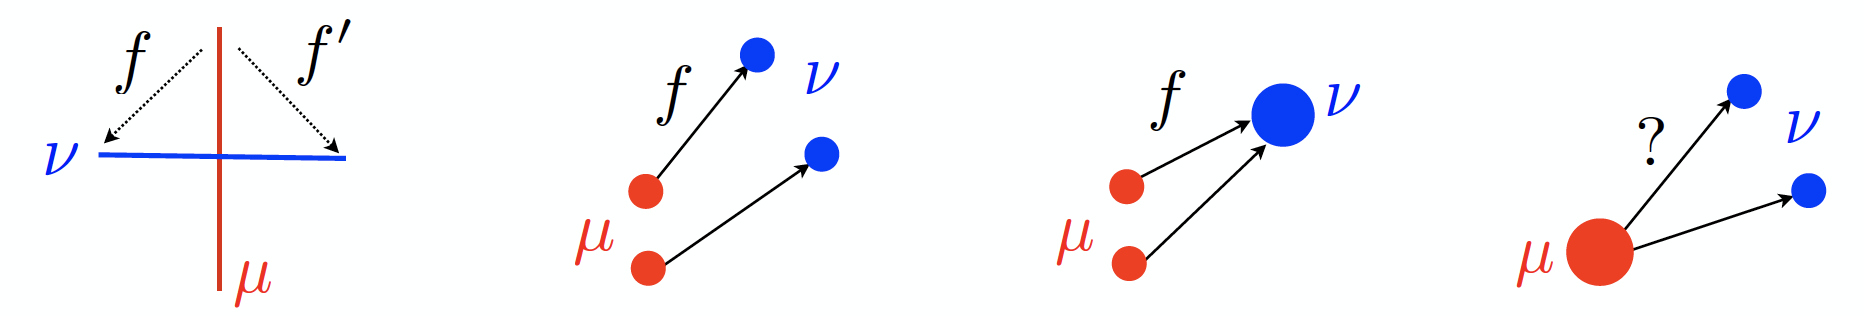
\includegraphics[width=0.9\linewidth]{fig/exist}
  \end{center}
\end{frame}
%----------------------------------------------------------------------------------------

\begin{frame}
  \frametitle{Kantorovich relaxation}
  \begin{center}
      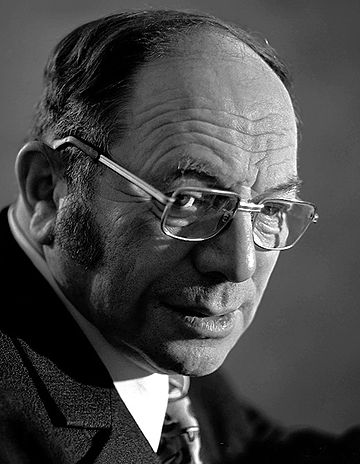
\includegraphics[width=0.3\linewidth]{fig/kanto} 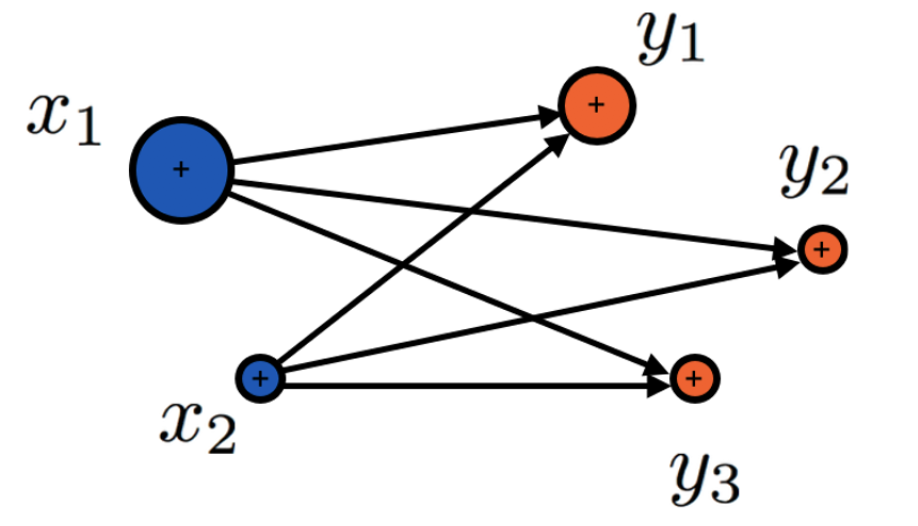
\includegraphics[width=0.6\linewidth]{fig/alloc}
  \end{center}
\begin{itemize}
\item Leonid Kantorovich (1912--1986), Economy nobelist in 1975, proposed a different formulation of the problem
\item with applications mainly for ressource allocation problems
\end{itemize}
\end{frame}
%----------------------------------------------------------------------------------------

\begin{frame}
  \frametitle{Kantorovich relaxation}

  \begin{center}
      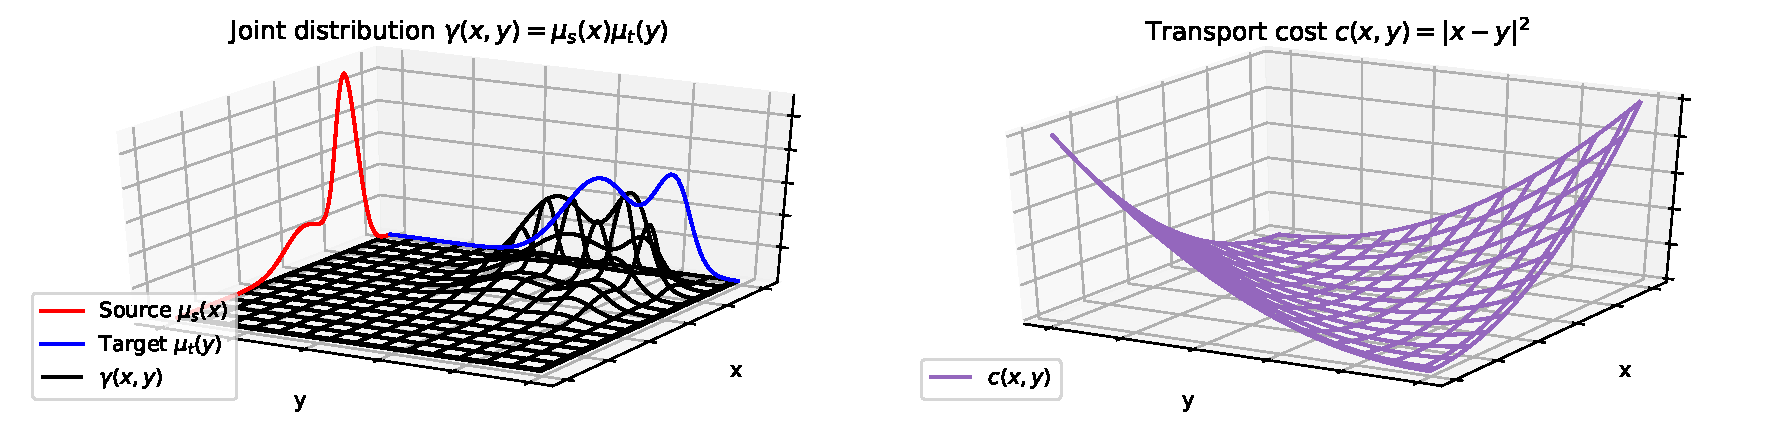
\includegraphics[width=0.9\linewidth]{fig/dist_kanto}
  \end{center}
$\red{\mu_{s}}=\sum_{i=1}^{n} a_{i} \delta_{x_{i}}$ and $\blue{\mu_{t}}=\sum_{j=1}^{m} b_{j} \delta_{y_{j}}$ on a commun ground space equipped with a distance

  \begin{itemize}

\item The Kantorovich formulation seeks for a probabilistic coupling $\pi \in \Pi(\mu_{s} \times \mu_{t})$ between
$\mu_{s}$ and $\mu_{t}$.
\item $\pi$ is a joint probability measure with prescribed
  marginals $\red{\mu_s}$ and $\blue{\mu_t}$.
\item Computes the Wasserstein distance :

\begin{equation}
\mathcal{W}_{p}(\red{\mu_{s}},\blue{\mu_{t}})=\bigg(\underset{\pi \in \Pi(\red{\mu_{s}},\blue{\mu_{t}})}{\min} \sum_{i,j} d(x_{i},y_{j})^{q} \pi_{i,j} \bigg)^{\frac{1}{p}}
\label{otwdiscrete}
\end{equation}

  \end{itemize}
Can be solved by linear programing
\end{frame}
%----------------------------------------------------------------------------------------

\begin{frame}
  \frametitle{Probabilistic couplings}
  
  The resulting coupling $\pi$ associates in a "fuzzy" way the points of the distributions.
  
  \begin{figure}
  \begin{center}
      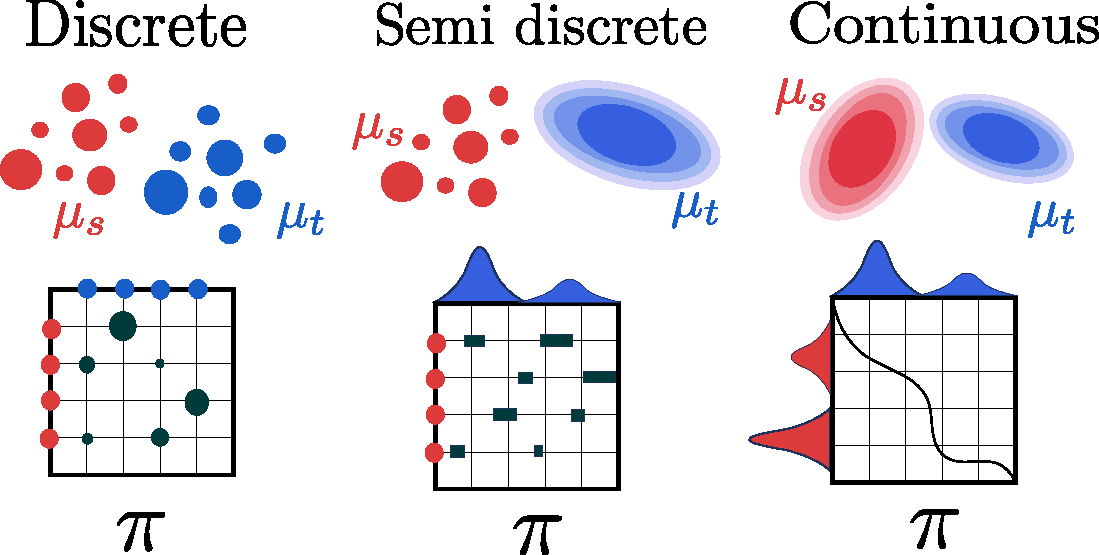
\includegraphics[width=0.9\linewidth]{fig/3ways.pdf}
  \end{center}
  \end{figure}
\end{frame}
%----------------------------------------------------------------------------------------


\begin{frame}
  \frametitle{Properties of Wasserstein distance}
  
  \begin{block}{The Wasserstein distance}
  \begin{itemize}
  \item The $p$-Wasserstein distance is always defined even for arbitrary measures even singular ones.
  \item The $p$-Wasserstein distance defines a metric over $\mathcal{P}(\Omega)$. It means that for $\alpha, \beta \in \mathcal{P}(\Omega), \mathcal{W}_{p}(\alpha,\beta)=0$ \textit{iff} $\alpha=\beta$ and $ \mathcal{W}_{p}$ satisfies the triangle inequality
  \item The $p$-Wasserstein distance is a weak metric, that means $(\alpha_{k})_{k}$ converges weakly (in law) to some $\alpha$ in $\mathcal{P}(\Omega)$ \textit{iff} $ \mathcal{W}_{p}(\alpha_{k},\alpha) \rightarrow 0$ as $k \rightarrow \infty$
  \end{itemize}
  \end{block}
  
  \pause
  
  The first point is one of the most interesting since "classical" distances (or divergences) are not even defined between discrete distributions. 
  
  \begin{itemize}
  \item The L2 norm can only be applied to continuous measures with a density with respect to a base measure
  \item The discrete $\ell_{2}$ norm requires that positions $(x_{i}, y_{j})$ take values in a predetermined dicrete set to work properly 
  \item Idem KL divergence is not defined if the supports of the measures does not overlap
  \end{itemize}


\end{frame}

%----------------------------------------------------------------------------------------

\begin{frame}
  \frametitle{Special case: 1D distribution}
We consider the case where $d(x,y=)|x - y|$ 
\begin{itemize}
\item if $x_{1} < x_{2}$ and $y_{1} < y_{2}$, it is easy to check that $d(x_{1},y_{1})+d(x_{2},y_{2})<d(x_{1},y_{2})+d(x_{2},y_{1})$
\item As such, any optimal transport plan respects the ordering of the elements, and the solution is given by the monotone rearrangement of $\mu_{s}$ onto $\mu_{t}$
\end{itemize}
This gives very simple algorithm to compute the transport in $O(N\log N)$, by sorting both $x_{i}$ and $y_{i}$ and summing the absolute values of differences.
  \begin{center}
      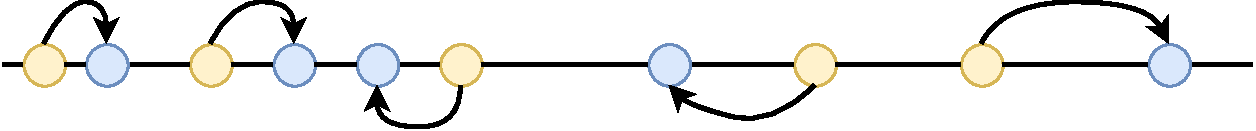
\includegraphics[width=0.9\linewidth]{fig/transp1D}
  \end{center}
\end{frame}


%----------------------------------------------------------------------------------------

\begin{frame}
  \frametitle{In the case $\Omega=\mathbb{R}^{d}$, $d(x,y)=\|x-y\|$ and $p=1$}

The optimal transport problem then aim to find $f \in \text{Lip}^1$ (set of 1-Lipschitz functions) as
\begin{equation}
\text{sup}_{f \in \text{Lip}^1} \int f d(\red {\mu_{s}} - \blue{\mu_{t}}) = \text{sup}_{f \in \text{Lip}^1} \mathbb{E}_{\x\sim\red {\mu_{s}} } [f(x)] - \mathbb{E}_{\y\sim\blue{\mu_{t}} } [f(y)]
\end{equation}
\begin{itemize}
\item known as {\bf Kantorovich-Rubinstein duality}
\item $\phi$ can be learnt as a neural network constrained to the set $\text{Lip}^1$.
\end{itemize}

\end{frame}


%----------------------------------------------------------------------------------------


\begin{frame}
  \frametitle{Optimal transport in Machine Learning}
  
Numerous applications for the Wasserstein distance :

 \begin{itemize}
 \item Learning with Wasserstein Loss \cite{2015arXiv150605439F} 
 \item Wasserstein GAN's \cite{arjovsky_wgan_2017}
\item Domain Adaptation \cite{courty2017optimal}
\item Image colorization \cite{ferradans2014regularized}, Dictionary Learning \cite{pmlr-v51-rolet16} ... 
 \end{itemize}


\end{frame}
%----------------------------------------------------------------------------------------



\subsection{Wasserstein GAN}
%----------------------------------------------------------------------------------------

\begin{frame}
\frametitle{Problem Setting \cite{arjovsky_wgan_2017}}
We consider a parametric family $(\mathbb{P}_{\theta})_{\theta \in \Theta}$ and a real data distribution $\mathbb{P}_{r}$. We want to solve :

\begin{equation}
\label{wassganeq}
\underset{\theta \in \Theta}{\text{min}} \  \mathcal{W}_{1}(\mathbb{P}_{r},\mathbb{P}_{\theta})
\end{equation}

Solving \eqref{wassganeq} is equivalent to find the closest distribution (\textit{w.r.t} the Wasserstein distance) amoung the given parametric family which fits the target distribution.

\end{frame}

%----------------------------------------------------------------------------------------

\begin{frame}
\frametitle{Problem Setting \cite{arjovsky_wgan_2017}}

The minimum of \eqref{wassganeq} is highly untractable but the Kantorovich-Rubinstein duality tells :

$$\mathcal{W}_{1}(\mathbb{P}_{r},\mathbb{P}_{\theta})= \underset{f \in \text{Lip}^1}\sup  \mathbb{E}_{\x\sim  \mathbb{P}_{r}} [f(x)] - \mathbb{E}_{y \sim \mathbb{P}_{\theta} } [f(y)]$$

If we rather consider $f \in \text{Lip}^K$ we end up with $K.\mathcal{W}_{1}(\mathbb{P}_{r},\mathbb{P}_{\theta})$

So, idea :

\begin{itemize}
\item $\mathbb{P}_{\theta}$ is coming from a neural network $g_{\theta}$ in the same way as traditional GAN's.
\item We consider another neural network $f_{w}$ called the \emph{critic} (alike a discriminator)
\end{itemize}

And we solve \eqref{wassganeq} \textit{via} :

\begin{equation}
\label{wassgan}
\underset{w}{\text{max}} \ \underset{\theta}{\text{min}} \  \underset{x \sim P_{r}}{\mathbb{E}}[f_{w}(x)]-\underset{z \sim p(z)}{\mathbb{E}}[f_{w}(g_{\theta}(z))]
\end{equation}

\end{frame}

%----------------------------------------------------------------------------------------

\begin{frame}
\frametitle{How do we find the function $f^{*}$ that solves the maximization problem ?}

How do we force $f_{w}$ to be K-Lip ??

\begin{itemize}
\item $f_{w}$ is parameterized by a neural network with weights $w$ lying in a compact space $\mathcal{W}$ imply that $f_{w}$ is K-Lip.
\item K only depend on $\mathcal{W}$
\item To force $f_{w}$ to be K-Lip we can clamp the weights to a fixed box (\textit{e.g} $\mathcal{W} = [-0.01,0.01]^{d}$ ) after each gradient update
\end{itemize}

\pause 

But :

\begin{itemize}
\item Weight clipping is a clearly terrible way to enforce a Lipschitz constraint
\item If the clipping parameter is large : long time for any weights to reach their limit, making it harder to train the critic till optimality
\item If the clipping is small : this can easily lead to vanishing gradients
\end{itemize}

\end{frame}


%----------------------------------------------------------------------------------------


\begin{frame}
\frametitle{Implementation of WGAN}

        \begin{algorithm}[H]   
            \begin{algorithmic}[1]
            \STATE{Require :$\alpha$ the learning rate. $c$, the clipping parameter. $m$, the batch size. $n_{c}$, the number of iterations of the critic per generator iteration}
             \STATE{Require : $w_{0}$, initial critic parameters. $\theta_{0}$, initial generator’s parameters.}
                \WHILE {$\theta_{g}$ has not converged}
                \FOR{$t=0,...,n_{c}$ }
                \STATE {sample minibatches $\{z_{1},...,z_{m}\}$  from noise prior $p(z)$}
                \STATE {sample minibatches $\{x_{1},...,x_{m}\}$  from data $\mathbb{P}_{r}$}
                \STATE {Update $f_{w}$  by ascending its stochastic gradient $$\nabla_{w} \frac{1}{m} \sum_{i=1}^{m} f_{w}(x_{i})- \frac{1}{m} \sum_{i=1}^{m} f_{w}(\g_{\theta_{g}}(z_{i}))$$}
                 %\STATE {$w \leftarrow w+ \alpha \text{RMSProp}(w,f_{w})$}
                 \STATE {$w \leftarrow \text{clip}(-c,c)$}
                \ENDFOR

                \STATE {sample minibatches $\{z_{1},...,z_{m}\}$  from noise prior $p(z)$}
                \STATE {Update the generator  by ascending its stochastic gradient $\nabla_{\theta_{g}} \frac{1}{m} \sum_{i=1}^{m}  f_{w}(\g_{\theta_{g}}(z_{i})) $}
                \ENDWHILE
            \end{algorithmic}
                      \caption{\label{gan} pseudo code of GAN}
        \end{algorithm}


\end{frame}
%----------------------------------------------------------------------------------------

%----------------------------------------------------------------------------------------

  \begin{frame}
    \frametitle{WGAN: the devil in the approximation}

\begin{block}{Neural network belonging to  $\text{Lip}^1$ ?}

  \begin{itemize}
    \item Not really! 
    \item It is actually the supremum over K-Lipschitz functions that is approximated by a neural network 
  \item Actually  {\bf not} equivalent to solve the optimal transport, but gradients are aligned.

  \end{itemize}
  
\end{block}\vspace{-2mm}


\begin{block}{Improved WGAN \cite{DBLP:journals/corr/GulrajaniAADC17}\vspace{-2mm}}
  $$
  \min_{\theta}\sup_{f \in \text{NN class}}\quad \mathbb{E}_{\x\sim \mathbb{P}_{r}}[ f(\x)] - \mathbb{E}_{\z\sim\mathcal{N}(0,\mathbf{I})} [f(g_{\theta}(\z))] + \lambda \mathbb{E}_{\x\sim \mathbb{P}_{r}}[ (||\nabla f(\x)||_2  - 1)^2 ]
  $$
  Relaxation of the constraint (for $W_1$ the gradient of the potential is $1$ almost everywhere).
\end{block}
  
  \end{frame}


\section{Autoencoder}


%----------------------------------------------------------------------------------------

\begin{frame}
\frametitle{Problem setting}

An autoencoder is a neural network that is trained to attempt to copy its input to its ouput. It has two parts :

\begin{itemize}
\item An encoder function $h_{\theta_{e}} : \mathcal{X} \rightarrow \mathcal{Z}$ that pushes the inputs $x$ in a smaller dimensional space.
\item A decoder function $g_{\theta_{d}} : \mathcal{Z} \rightarrow \mathcal{X}$ that reconstructs from the low dimensional space to the initial space
\end{itemize}

Very generally autoencoders aim at solving  : 
\begin{equation}
\label{autoencodergeneral}
%\underset{\theta_{e},\theta_{d}}{\text{min}} \ \underset{x \sim \mathbb{P}_{r}}{\mathbb{E}}[L(x,g_{\theta_{d}}(h_{\theta_{e}}(x)))]
\underset{\theta_{e},\theta_{d}}{\text{min}} \ \underset{x \sim \mathbb{P}_{r}}{\mathbb{E}}[L(x,g_{\theta_{d}},h_{\theta_{e}})]
\end{equation}

\end{frame}

%----------------------------------------------------------------------------------------

\begin{frame}
\frametitle{Traditional autoencoders}

The most classical autoencoders are \emph{undercomplete autoencoders} : the latent space has a smaller dimension $\text{dim}(\mathcal{Z}) << \text{dim}(\mathcal{X})$ (typically subset of $\mathbb{R}^{d}$ with $d$ small) : 


\begin{equation}
\label{autoencoderclassical}
\underset{\theta_{e},\theta_{d}}{\text{min}} \ \underset{x \sim \mathbb{P}_{r}}{\mathbb{E}}[L(x,g_{\theta_{d}}(h_{\theta_{e}}(x)))]
\end{equation}

\begin{itemize}
\item $L$ is chosen to be a reconstruction error as $\ell_{2}$ error
\item Forces the network to acts as the indentity. The latent space acts as a dimentional reduction of $\mathcal{X}$.
\item When the decoder is linear and L is the mean squared error, an undercomplete autoencoder learns to span the same subspace $\mathcal{Z}$ as PCA.
\end{itemize}


\begin{figure}
\label{autoencodeurfig}
\centering
    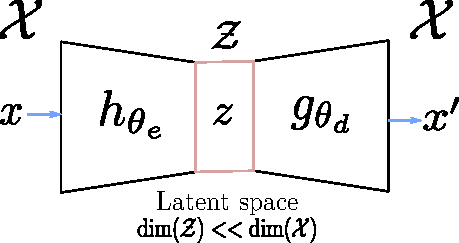
\includegraphics[width=0.5\textwidth]{fig/autoencoder.pdf}
  %\caption{$h_{\theta_{e}}$ pushes the inputs $x$ in the latent space. $g_{\theta_{d}}$ reconstructs from the low dimensional space to the initial space}
\end{figure}

\end{frame}

%----------------------------------------------------------------------------------------

\begin{frame}
\frametitle{Learning manifolds}

\begin{figure}
  \begin{center}
    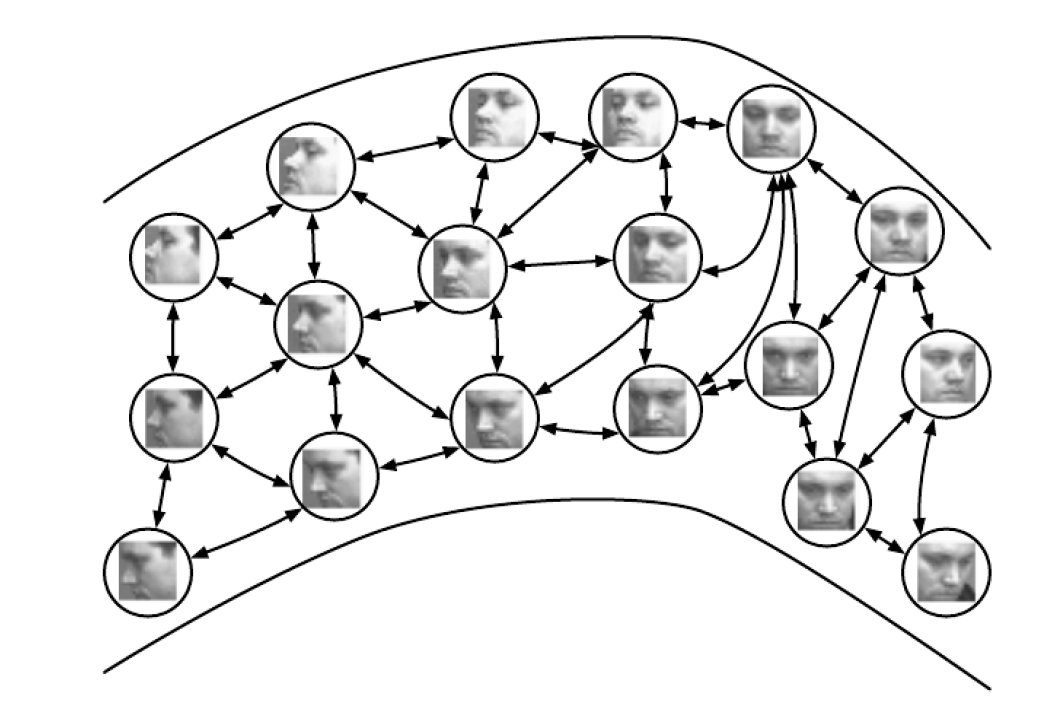
\includegraphics[width=0.8\textwidth]{fig/learning_manifolds.png}
  \end{center}
 \caption{Non-parametric manifold learning procedures build a nearest neighbor graph in which nodes represent training examples a directed edges indicate nearest neighbor relationships. The coordinate system associates each training example with a real-valued vector position in the embedding $\mathcal{Z}$. \cite{Gong:2000:DVI:572750}}
\end{figure}

\end{frame}
%----------------------------------------------------------------------------------------


\begin{frame}
\frametitle{Dimensionality reduction}
\begin{itemize}
\item Lower-dimensional representations can improve performance on many tasks, such as classification.
\item Models of smaller spaces consume less memory and runtime.
\item Interesting for \textit{e.g} in information retrieval : finding entries in a database that resemble a query entry. We can store a full complicated database in a hash table mapping binary code vectors to entries and do fast queries.
\end{itemize}


\end{frame}

%----------------------------------------------------------------------------------------

\begin{frame}
\frametitle{Many variants}

\begin{itemize}
\item Regularized autoencoders :  if $\text{dim}(\mathcal{Z})\approx \text{dim}(\mathcal{X})$ 
\begin{itemize}
\item In this case classical autoencoders usually fail to learn anything useful.
\item Regularized autoencoders  use a loss function that encourages the model to have other properties besides the ability to copy its input to its output : sparsity of the representation, smallness of the derivative of the representation, and robustness to noise or to missing inputs
\item See VAE
\end{itemize}
\item Sparse autoencoders :  the learning process aim at minimizing $$L(x,g_{\theta_{d}}(h_{\theta_{e}}(x))) + \Omega(z)$$
\begin{itemize}
\item $ \Omega$ is a regularization function in the latent space $z=h_{\theta_{e}}(x)$.
\item  Sparse autoencoders are typically used to learn features for another task such as classification
\end{itemize}
\end{itemize}


\end{frame}
%----------------------------------------------------------------------------------------



\begin{frame}
\frametitle{Many variants}

\begin{itemize}
\item Denoising autoencoders : the learning process aim at minimizing $$L(x,g_{\theta_{d}}(h_{\theta_{e}}(\tilde{x})))$$
\begin{itemize}
\item $\tilde{x}$ is a copy of $x$ that has been corrupted by some form of noise.
\item Denoising training forces $h_{\theta_{e}}$ and $g_{\theta_{d}}$ to implicitly learn the structure of $\mathbb{P}_{r}$
\end{itemize}
\item Contracting autoencoders : the learning process aim at minimizing $$L(x,g_{\theta_{d}}(h_{\theta_{e}}(x))) + \Omega(z,x)$$
\begin{itemize}
\item $\Omega(z,x) = \lambda \sum_{i} \| \nabla_{x} h_{\theta_{e}}(x)_{i} \|$
\item This forces the model to learn a function that does not change much when $x$ changes slightly
\item It forces the autoencoder to learn features that capture information about the training distribution.
\end{itemize}
\end{itemize}


\end{frame}



%----------------------------------------------------------------------------------------


\section{Variationnal autoencoder}

%----------------------------------------------------------------------------------------



\begin{frame}
\frametitle{The probabilistic point of view}

Encoder and decoder previously defined can be seen as distributions : 
\begin{itemize}
\item From an input $x \in \mathcal{X}$ of the data and from parameters $\theta_{e}$, the encoder outputs a hidden representation $z \in \mathcal{Z}$. This process defines a conditional distribution $q_{\theta_{e}}(z|x)$
\item In the same way from parameters $\theta_{d}$ and a hidden representation $z \in \mathcal{Z}$ the decoder output a point $x$ in the space $\mathcal{X}$. This process defines a conditional distribution $p_{\theta_{d}}(x|z)$
\end{itemize}


In the digit example with each pixel as $0$ and $1$ : the probability distribution of a single pixel can be then represented as a Bernoulli distribution. 
\begin{itemize}
\item The encoder gets as input the latent representation of a digit $z$ and outputs 784 Bernoulli parameters, one for each of the 784 pixels in the image.
\item  The decoder decodes the real-valued numbers in $z$ into 784 real-valued numbers between $0$ and $1$.
\end{itemize}


\end{frame}

%----------------------------------------------------------------------------------------

\begin{frame}
\frametitle{Problem setting}

The basic idea of VAE is to force the distribution $q_{\theta_{e}}(z|x)$ coming from the encoder to follow a certain distribution $p(z)$ (typically a normal distribution) in order to generate samples.

In this case we want to minimize \textit{w.r.t} $\theta_{e}$ and $\theta_{d}$ the following quantity  :

\begin{equation}
\label{vaeeq}
 \underset{}{} \underset{z \sim q_{\theta_{e}}(z|x)}{-\mathbb{E}}[\log(p_{\theta_{d}}(x|z))] + \text{KL}(q_{\theta_{e}}(z|x) || p(z))
\end{equation}
for  $x \sim \mathbb{P}_{r}$

\begin{figure}
  \begin{center}
    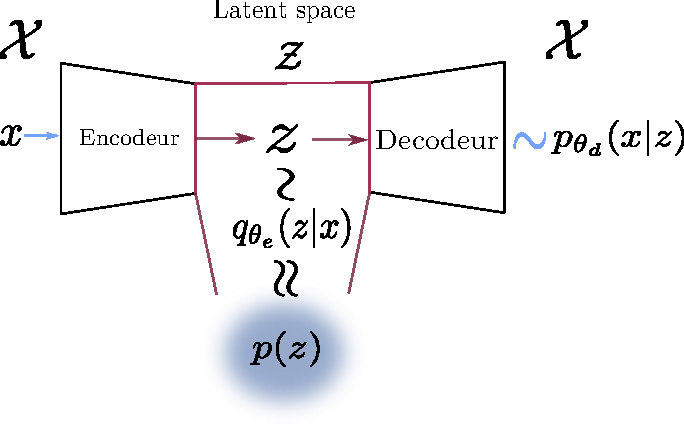
\includegraphics[width=0.7\textwidth]{fig/vae.pdf}
  \end{center}
\end{figure}

\end{frame}

%----------------------------------------------------------------------------------------

\begin{frame}
\frametitle{Problem setting}


\begin{itemize}
\item $\underset{z \sim q_{\theta_{e}}(z|x)}{-\mathbb{E}}[\log(p_{\theta_{d}}(x|z))]$ is the reconstruction loss : encourages the decoder to learn to reconstruct the data $\mathbb{P}_{r}$.
\item $\text{KL}(q_{\theta_{e}}(z|x) || p(z))$ is the regularization term : it measures how much information is lost when using $q_{\theta_{e}}(z|x)$ to represent $p(z)$. It encourages $q_{\theta_{e}}(z|x)$ to be equal to $p(z)$.
\end{itemize}

We usually choose $p(z)=\mathcal{N}(0,I)$. Once the network is trained it is easy to generate samples : pick a $z\sim \mathcal{N}(0,I)$ (easy) a feed the learned generator $p_{\theta_{d}}(x|z)$ with it.

\end{frame}
%----------------------------------------------------------------------------------------

\begin{frame}[allowframebreaks]
        \frametitle{References}
        \bibliographystyle{amsalpha}
        \bibliography{./biblio}
\end{frame}
%----------------------------------------------------------------------------------------


\end{document}